% !TEX root = ../thesis-sample.tex

\chapter{Autonomous Exploration in Complex 3D Space} \label{chap:ae3Dcomplex}

This chapter extends the autonomous exploration scheme to complex 3D environments. Unlike Chapter \ref{chap:ae2D} where exploration was applied in 2D, or Chapters \ref{chap:ae3Dsimple} and \ref{chap:multivehicle} where exploration was confined to a single height in vertically-uniform environments, this chapter proposes a completely 3D exploration approach for complex environments. This proposed approach is designed for rooms with complicated features and places with changing and uncertain terrain such as Mars.

\section{Exploration in 3D}

In this section, we propose how multiple measurement rays in 3D can determine map information gain from a pose candidate. Then, we show how a collision-free trajectory is determined with a 3D Dijkstra's search. Finally, we combine 3D information gain and travel costs into a single optimization.

\subsection{Map Information Gain in 3D}

The expected entropy for an arbitrary 1D ray spanning 3D space can be calculated with \refeqn{DiscExpEntropyRay} and \refeqn{ProbMeas} in a computationally tractable manner. However, computing the expected entropy from multiple rays simultaneously has exponential complexity, and is therefore computationally intractable. Additionally, numerous rays of a single scan commonly intersect the same grid cells, making consideration of \emph{every} measurement ray unnecessary.

Instead of considering expected entropy from a complete scan, we propose a real-time solution that selects sample measurements to determine an optimal attitude at each candidate pose and the associated map information gain, similar to how the scan information gain is found in Section \ref{sec:OptimalPose2DMap}. We assume the vehicle is capable of level flight, so the third axes of the world and body are aligned (Figure \ref{fig:transforms}), so $R_c$ can be expressed as
\begin{align*}
R_c=\begin{bmatrix}
\cos\psi & -\sin\psi & 0
\\
\sin\psi & \cos\psi & 0
\\
0 & 0 & 1
\end{bmatrix}, \quad 0\leq\psi<2\pi,
\end{align*}
where $\psi$ represents the angle about the third body-fixed axis. The direction of a 3D measurement may also have a nonzero component in the vertical direction. This is achieved by rotating the sensor frame angle $\theta$ about the second sensor-fixed axis,
\begin{align*}
R_{c,\text{sensor}}=\begin{bmatrix}
\cos\theta & 0 & \sin\theta
\\
0 & 1 & 0
\\
-\sin\theta & 0 & \cos\theta
\end{bmatrix}, \quad -\frac{\pi}{2}\leq\theta\leq\frac{\pi}{2}.
\end{align*}
Combining these two rotation matrices, the measurement $z$ with depth $\norm{z}$ is expressed with respect to a frame fixed to the world as
\begin{align}
z(\psi,\theta)=\begin{bmatrix}\cos\theta\cos\psi & -\sin\psi & \cos\psi\sin\theta
\\
\cos\theta\sin\psi & \cos\psi & \sin\psi\sin\theta
\\
-\sin\theta & 0 & \cos\theta
\end{bmatrix}
\begin{bmatrix}
\norm{z} \\ 0 \\ 0
\end{bmatrix}
=
\begin{bmatrix}
\cos\theta\cos\psi
\\
\cos\theta\sin\psi
\\
-\sin\theta
\end{bmatrix}\norm{z}.
\end{align}
In short, unit vectors are acquired via Euler angles within certain sensor limits.

% trim={<left> <lower> <right> <upper>}

\begin{figure}[!t]
	\centering
	\begin{subfigure}[t]{0.3\columnwidth}
           	\centering
          	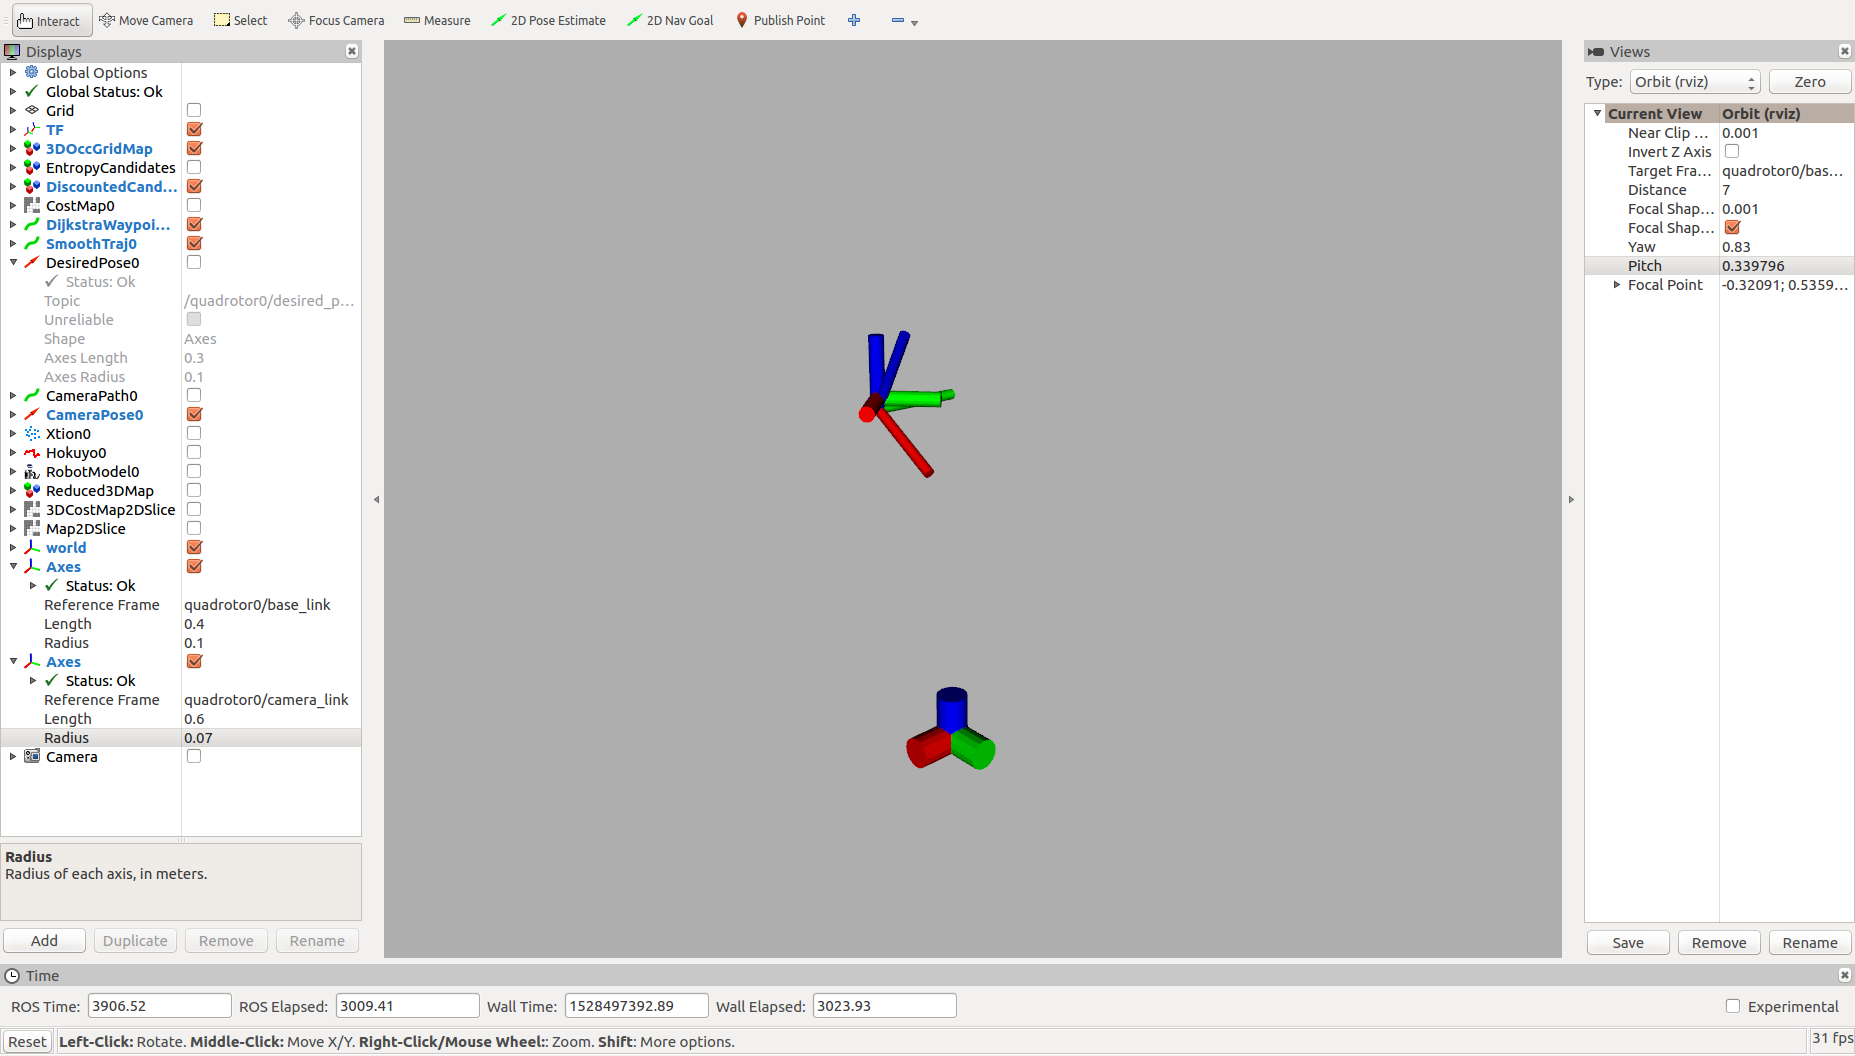
\includegraphics[trim = {21cm 5cm 20cm 5cm}, clip, height=1.0\textwidth]{mars_general.png}
        		\caption{General View}
    	\end{subfigure}
    	\begin{subfigure}[t]{0.3\columnwidth}
           	\centering
          	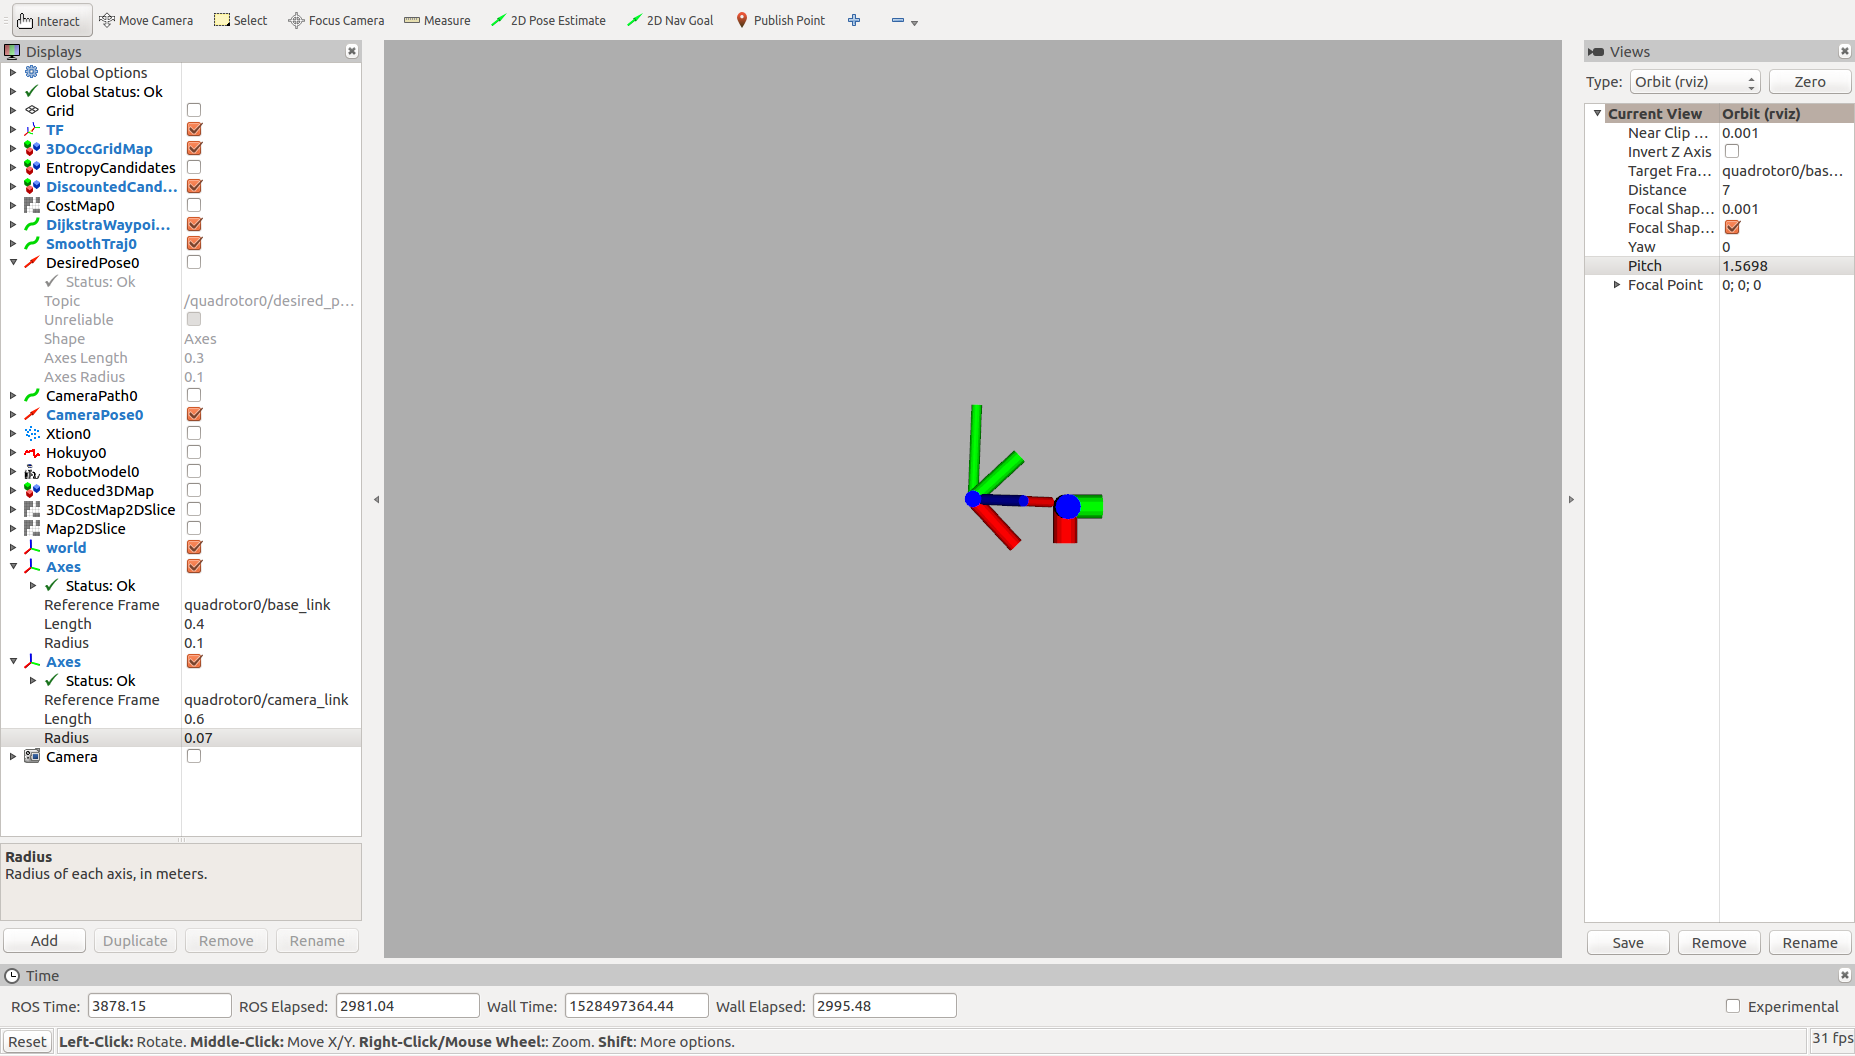
\includegraphics[trim = {25cm 6cm 16cm 4cm}, clip, height=1.0\textwidth]{mars_psi.png}
        		\caption{$\psi$ Rotation}
    	\end{subfigure}
	\begin{subfigure}[t]{0.3\columnwidth}
           	\centering
          	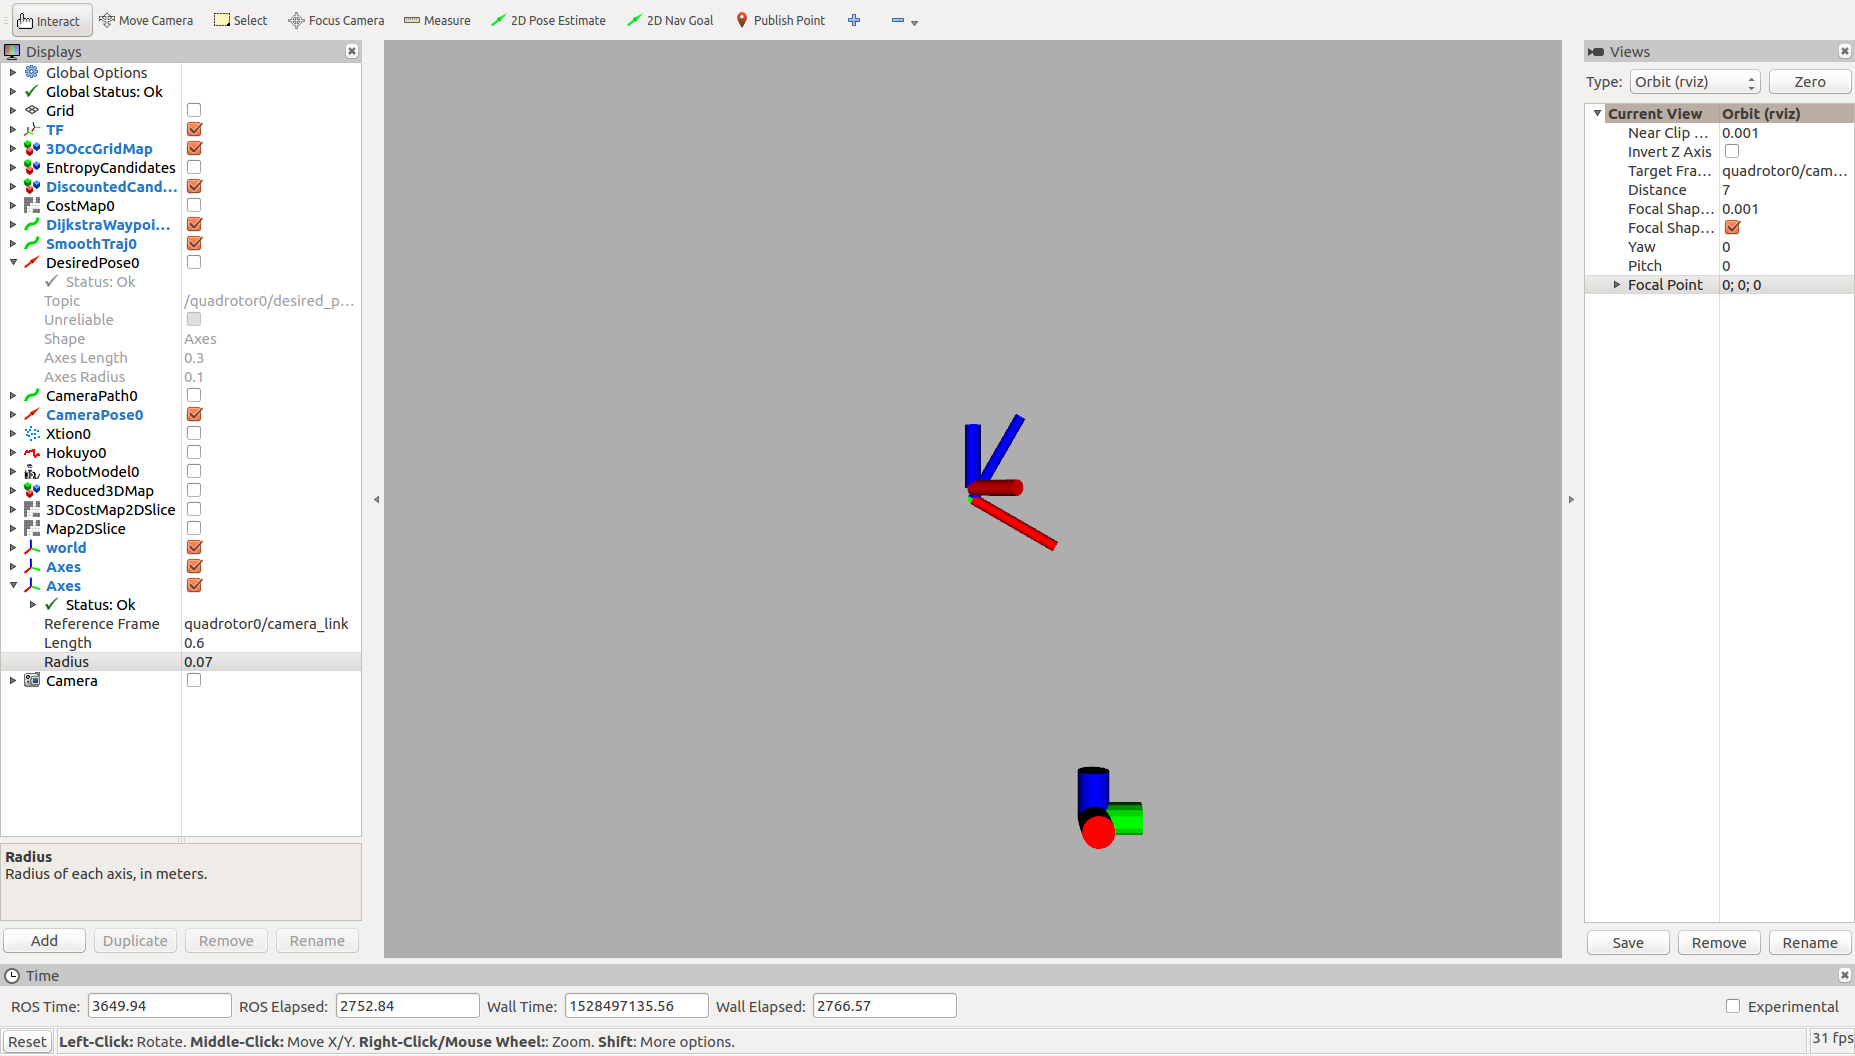
\includegraphics[trim = {23cm 4cm 17cm 6cm}, clip, height=1.0\textwidth]{mars_theta.png}
        		\caption{$\theta$ Rotation}
    	\end{subfigure}
%\includegraphics[width=2.5in]{myfigure}
% where an .eps filename suffix will be assumed under latex, 
% and a .pdf suffix will be assumed for pdflatex; or what has been declared
% via \DeclareGraphicsExtensions.
\caption{The three frames are shown with three axes (red: first axis, green: second axis, blue: third axis). The Mars frame (short and thick) is fixed to the planet. The body-fixed frame (medium thickness and length) is fixed to the camera frame (long and narrow). The rotation of $\psi$ (b) represents the fixed camera yaw rotation and $\theta$ (c) represents the downward angle of the camera to capture the surface of Mars below the flying robot.}
\label{fig:transforms}
\end{figure}


Next, we show how multiple 3D measurements provide an estimate for information gain. Let $\Psi$ and $\Theta$ be the angular ranges for the sensor FOV in the horizontal and vertical directions, respectively. Within the sensor FOV, we select sample measurements for evaluating their expected information gains. Let the number of sample measurements be $n_\psi$ and $n_\theta$ for horizontal and vertical rotations, respectively. Since $R_c$ and the FOV are known, the set of sample measurement rays, namely $\mathcal{Z}(R_c)$, is known as well. Then, the expected information gain for a single measurement ray $z$ from candidate position $x_c$ and attitude $R_c$ is the negative expected entropy change,
\begin{align}
\label{eqn:Iray}
\mathcal{I}&_\text{ray}(x_c,R_c,\psi,\theta)\nonumber\\&=
\begin{cases}
H(P(r))-\text{E}[H(P(r|x_c,z(\psi+\tilde{\psi},\theta+\tilde{\theta})))], & \mbox{if } z(\psi+\tilde{\psi},\theta+\tilde{\theta})\in\mathcal{Z}(R_c), \\ 
0,                                                                                    & \mbox{otherwise},
\end{cases}
\end{align}
where the mounting yaw $\tilde{\psi}$ and pitch $\tilde{\theta}$ of the sensor is a fixed rotation in the horizontal and vertical directions, respectively in that order, such that $-\pi<\tilde{\psi}\leq\pi$ and $-\frac{\pi}{2}+\frac\Theta2\leq\tilde{\theta}\leq\frac{\pi}{2}-\frac\Theta2$. A positive $\tilde{\theta}$ corresponds to rotating the depth sensor from a forward direction to a downward direction toward the ground below. The expected information gain for the full scan is the summation of expected information gains for individual rays
\begin{align}
\label{eqn:Iscan}
\mathcal{I}_\text{scan}(x_c,R_c)=\sum_{i_\psi=1}^{n_\psi}\sum_{i_\theta=1}^{n_\theta}\mathcal{I}_\text{ray}\left(x_c,R_c,\frac{(2i_\psi-n_\psi-1)\Psi}{2n_\psi},\frac{(2i_\theta-n_\theta-1)\Theta}{2n_\theta}\right).
\end{align}

Finally, \refeqn{Iscan} is computed for $n_\psi$ possible attitudes when the robot is at location $x_c$, one corresponding to each yaw angle $\psi$. Then, the optimal attitude at $x_c$ is
\begin{align}
\label{eqn:RcStar}
R_c^*=\argmax_{R_c} \mathcal{I}_\text{scan}(x_c,R_c).
\end{align}

In short, the expected information gain from each possible measurement ray is obtained using predicted entropy from \refeqn{DiscExpEntropyRay} and \refeqn{ProbMeas}. Then the expected information gain from all possible scans at a candidate location is calculated from \refeqn{Iray} and \refeqn{Iscan}. Finally, the optimal attitude at this candidate location is found using \refeqn{RcStar}.

\subsection{Collision-Free Trajectory in 3D}

Next, we present a fairly straightforward application of Dijkstra's search to 3D occupancy grid mapping. First we reduced the number of grid cells to cubic blocks large enough for a robot to fit completely inside. Based on the occupancy probability of these blocks and their neighbors, we determine which cells are reachable, and what are their travel costs by building a cost map based on Dijkstra's algorithm.

Here we describe how a reduced map is generated for collision avoidance and motion planning. If the largest edge-to-edge distance of the robot, namely $\rho$, is not larger than the 3D grid cell size $\alpha$, this step is unnecessary. Let $k\geq1$ be an integer such that $k\alpha\geq\rho$ and $(k-1)\alpha<\rho$, i.e., $k$ is the minimum number of grid cells in each dimension capable of fully-enclosing the robot inside this cube. Then, we decompose the complete probabilistic 3D into map $ m_\text{reduced}$, which is composed of larger cubic cells that encompass $k^3$ cells from map $ m$. Let $\mathbf{m}_{\text{reduced},k}$ denote the $k$-th cell of $ m_\text{reduced}$ being occupied, and let $a_k\subset m$ be those $k^3$ cells from $ m$ composing this larger cell. Then, we apply the same criteria as \refeqn{CombinationProjection2DMap} to obtain the probability of $\mathbf{m}_{\text{reduced},k}$ in 3D,

\begin{align}
\label{eqn:Proj3DMapComb}
P(\mathbf{m}_{\text{reduced},k})= 
\begin{cases}
    \max_{i\in a_k}{P(\mathbf{m}_i)},	&\text{if} \ \max_{i\in a_k}{P(\mathbf{m}_i)}\geq P_\text{thresh},\\
    \min_{i\in a_k}{P(\mathbf{m}_i)},	& \text{otherwise},
\end{cases}
\end{align}
where initial probability is $0<P_\text{init}<1$ and the threshold probability is constrained to $P_\text{init}<P_\text{thresh}<1$. This approach uses probabilities that have changed from $P_\text{init}$, and favors occupied cells to avoid risking collisions.

Next, we show how $\mathbf{m}_{\text{reduced},k}$ is used in Dijkstra's search for collision avoidance and motion planning. Defining $0<P_\text{coll}<1$ as the acceptable probability of collision, every grid cell of $ m_\text{reduced}$ is considered a safe and unvisited node if its occupancy probability, and the occupancy probabilities of its neighbors (sharing a face, edge, or corner), are below $P_\text{coll}$. A cost map is built from the starting robot location by neighboring nodes, where the cost to travel to another node is based on Euclidian distance: a cell sharing a face is $\alpha$ away, a cell sharing an edge is $\sqrt2\alpha$ away, and a cell sharing a corner is $\sqrt3\alpha$ away. Generating a cost map for all reachable cells in $\mathbf{m}_{\text{reduced},k}$ provides a collision-free travel cost for all reachable candidate pose locations. Once an optimal pose is selected, the path is easily found from the cost map using steepest descent.


\subsection{Optimal 3D Pose}

Here we present how an optimal pose is selected based on information gains at optimal attitudes and known collision-free travel costs. This process is similar to prior the autonomous exploration proposed in earlier chapters, with a few minor differences.

The proposed 3D autonomous exploration follows a receding-horizon framework, and uses a bump function \refeqn{BumpFunIncreasing}--\refeqn{BumpFun} to account for travel distance. The only difference is that the start of the bump function $B_1(d)=f_\text{max}$, illustrated in Figure \ref{fig:recedingHorizonBumpFun}). This change, though minor, avoids the possible scenario where a robot repeatedly alternates between neighboring candidates with similar expected information gains.
Then, we incorporate expected information gain and travel costs into a unified optimization. Given $d(x_c)$ from Dijkstra's cost map, the optimal candidate location is
\begin{align}
\label{eqn:CandidateLocationOptimization}
x_c^*=\argmax_{x_c}\mathcal{I}_\text{scan}(x_c,R_c^*)\mathcal B(d(x_c)),
\end{align}
and therefore the optimal pose is $X_c^*=\braces{x_c^*,R_c^*}$.

	\begin{figure}
	\vspace*{-0.3\columnwidth}
		\centerline{
			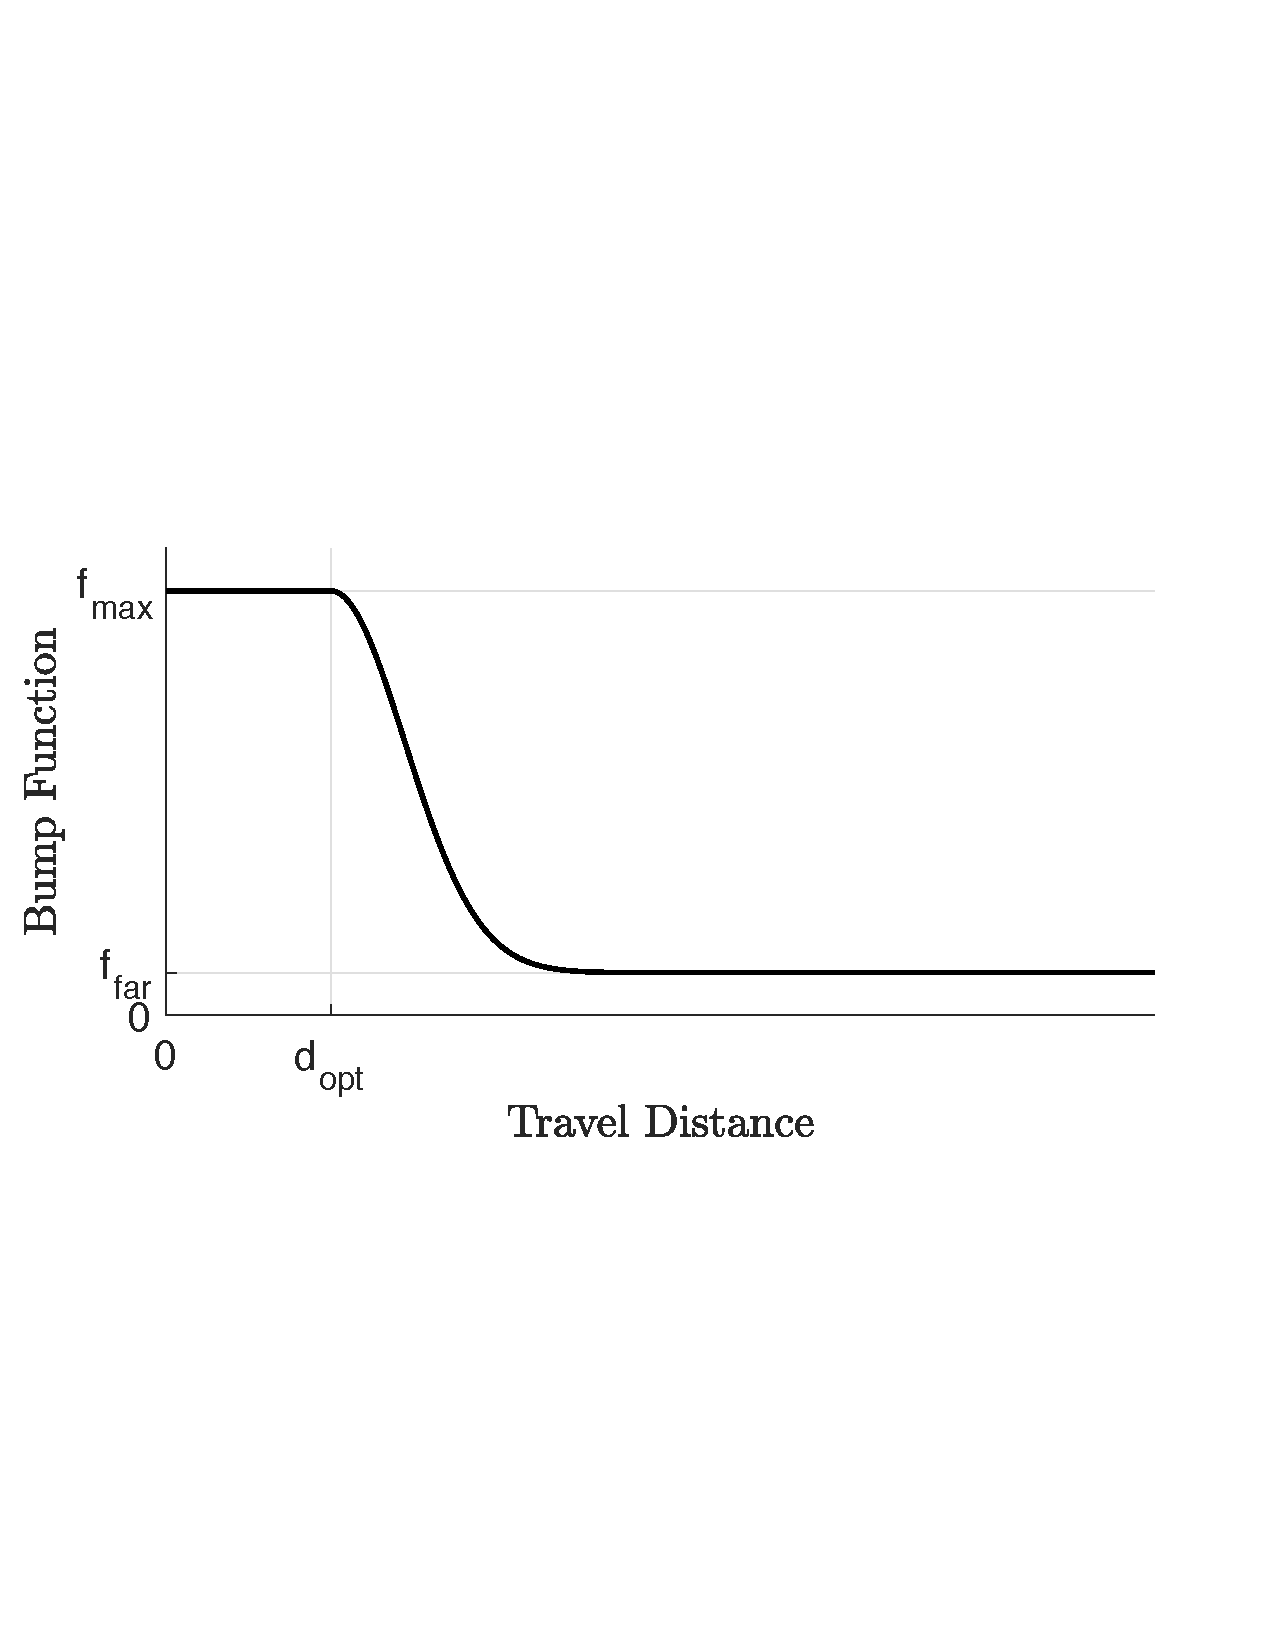
\includegraphics[width=0.6\columnwidth]{recedingHorizonBumpFunFlattened.pdf}
		}
	\vspace*{-0.25\columnwidth}
		\caption{The bump function is multiplied to the objective function of \refeqn{CandidateLocationOptimization} to prioritize local trajectories to avoid traversals across the map, where travel costs are determined using Dijkstra's algorithm. However, there is no time wasted up to $d_\text{opt}$ because this distance may be achieved in the minimum exploration computation time.}
		\label{fig:recedingHorizonBumpFun}
	\end{figure}
	
In conclusion, every reachable candidate pose is considered for its optimal attitude, which is found using sample rays spanning 3D space. The travel costs, acquired from Dijkstra's search, serve as input for the bump function, which prioritizes local trajectories to avoid costly map traversals. Then, the optimal candidate location is selected to maximize a combination of expected information gain and travel cost.



\section{Numerical Simulation}
In this section, we demonstrate the efficacy of the proposed 3D mapping and autonomous exploration with a simulated Mars environment. First we cover the parameters, then compare results using two different maps for entropy prediction.

\subsection{Mars Parameters}

A 3D environment of Mars is simulated in Gazebo. A height map~\cite{mapaplanet} is used to generate a contoured surface, and the corresponding picture of Mars is draped over this contour, shown in Figure \ref{fig:MarsGazebo}. A 3D laser scanner is also simulated in Gazebo. In the horizontal direction, the sensor has limits $\Psi=120^{\circ}$ with a total of $1000$ measurement rays inside, the sensor is fixed at angle $\tilde{\psi}=45^{\circ}$, and $n_\psi=16$ sample measurements are used. In the vertical direction, the sensor also has limits $\Theta=120^{\circ}$ with a total of $1000$ measurement rays inside, but the sensor is fixed at angle $\tilde{\theta}=30^{\circ}$, and $n_\psi=7$ sample measurements are used. These ray samples are taken from each candidate location, which are separated $1$ m apart in each of the $3$ dimensions.

% trim={<left> <lower> <right> <upper>}


\begin{figure}[!t]
	\centering
	\begin{subfigure}[t]{0.3\columnwidth}
           	\centering
          	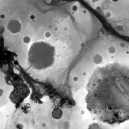
\includegraphics[height=0.9\textwidth]{mars_heightmap.png}
        		\caption{Height Map}
    	\end{subfigure}
    	\begin{subfigure}[t]{0.3\columnwidth}
           	\centering
          	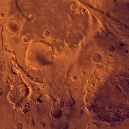
\includegraphics[height=0.9\textwidth]{mars_colormap.png}
        		\caption{Color Map}
    	\end{subfigure}
    	\begin{subfigure}[t]{0.3\columnwidth}
           	\centering{
          	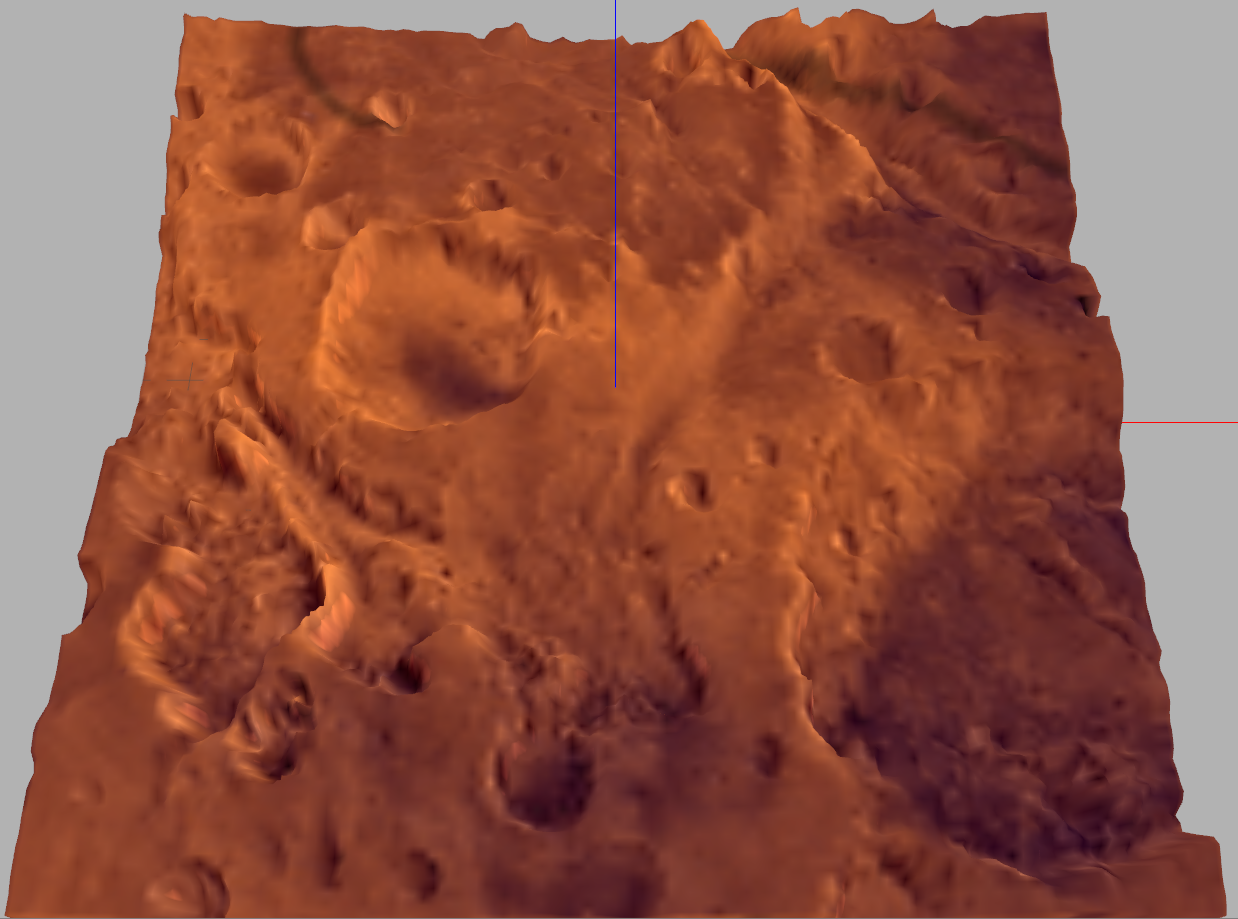
\includegraphics[height=0.9\textwidth]{mars_gazebo_full_lighting.png}}
        		\caption{Gazebo Environment}
    	\end{subfigure}
\caption{The height map (a) and color map (b) are combined in the Gazebo simulator (c) to model a Mars environment. The robot captures the simulated environment to generate an occupancy grid map.}
\label{fig:MarsGazebo}
\end{figure}

The map parameters are also important to the success of the exploration. The full map has dimensions $20$ m $\times$ $20$ m $\times$ $5$ m in the Mars-fixed frame, with cell edge length $\alpha=0.075$ m. The reduced map for collision-avoidance and motion planning has cells $k=3$ times the size ($0.225$ m), so $k^3=27$ cells are considered in \refeqn{Proj3DMapComb}. The bump functions use $f_\text{max}=1.0$, $f_\text{far}=0.1$, and $\beta=0.1$ to account for travel costs with \refeqn{BumpFun}. The receding horizon optimal time $d_\text{opt}$ is based on a fixed robot velocity of $0.25$ m/sec and the computation time varies from $1.8$ sec to $2.5$ sec.

\subsection{Mars Results}

The simulation was run twice. Case 1 was as described in this paper. Case 2 was identical to Case 1, except the reduced map $ m_\text{reduced}$ is used when computing \refeqn{Iscan}. Case 2 is largely inspired by the promising experimental results covered in Section \ref{sec:QuadrotorNRL}, where a projected map based on the same criteria as \refeqn{Proj3DMapComb} proved effective for level flight. The resulting occupancy grid maps for Cases 1 and 2 are shown in Figures \ref{fig:mars3DogmCase1} and \ref{fig:mars3DogmCase2}, respectively. A video of Case 1 can be found at \href{https://youtu.be/FrBcL2UMW9w}{\WriteBlue{https://youtu.be/FrBcL2UMW9w}}, and close-up pictures from Case 2 are shown in Figure \ref{fig:marsZoomedIn}. The complete map entropies for both cases are illustrated in Figure \ref{fig:mars3Dentropy}.


\begin{figure}[!t]
	\centering
	\begin{subfigure}[t]{0.49\columnwidth}
           	\centering
          	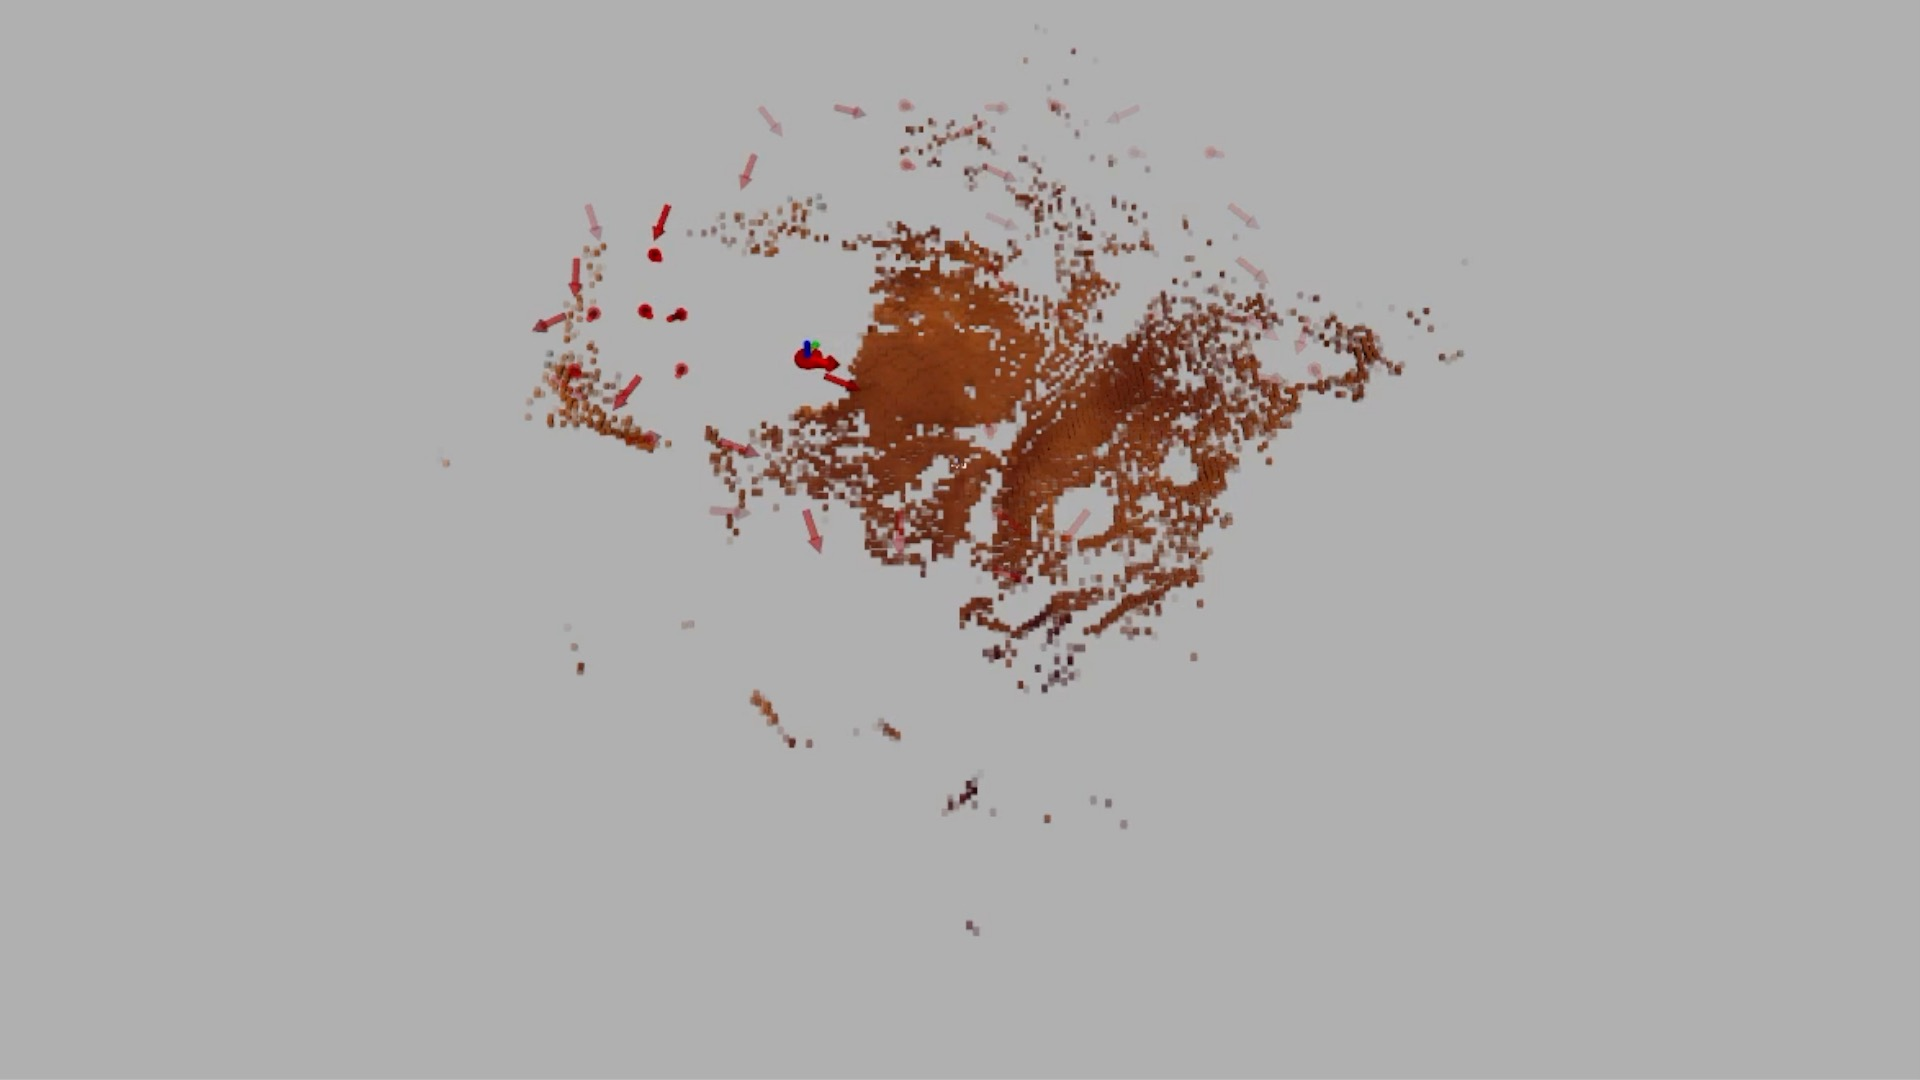
\includegraphics[height=0.5\textwidth]{FullMarsMap30sec.jpg}
        		\caption{$30$ sec}
		\vspace*{0.025\textwidth}
    	\end{subfigure}
    	\begin{subfigure}[t]{0.49\columnwidth}
           	\centering
          	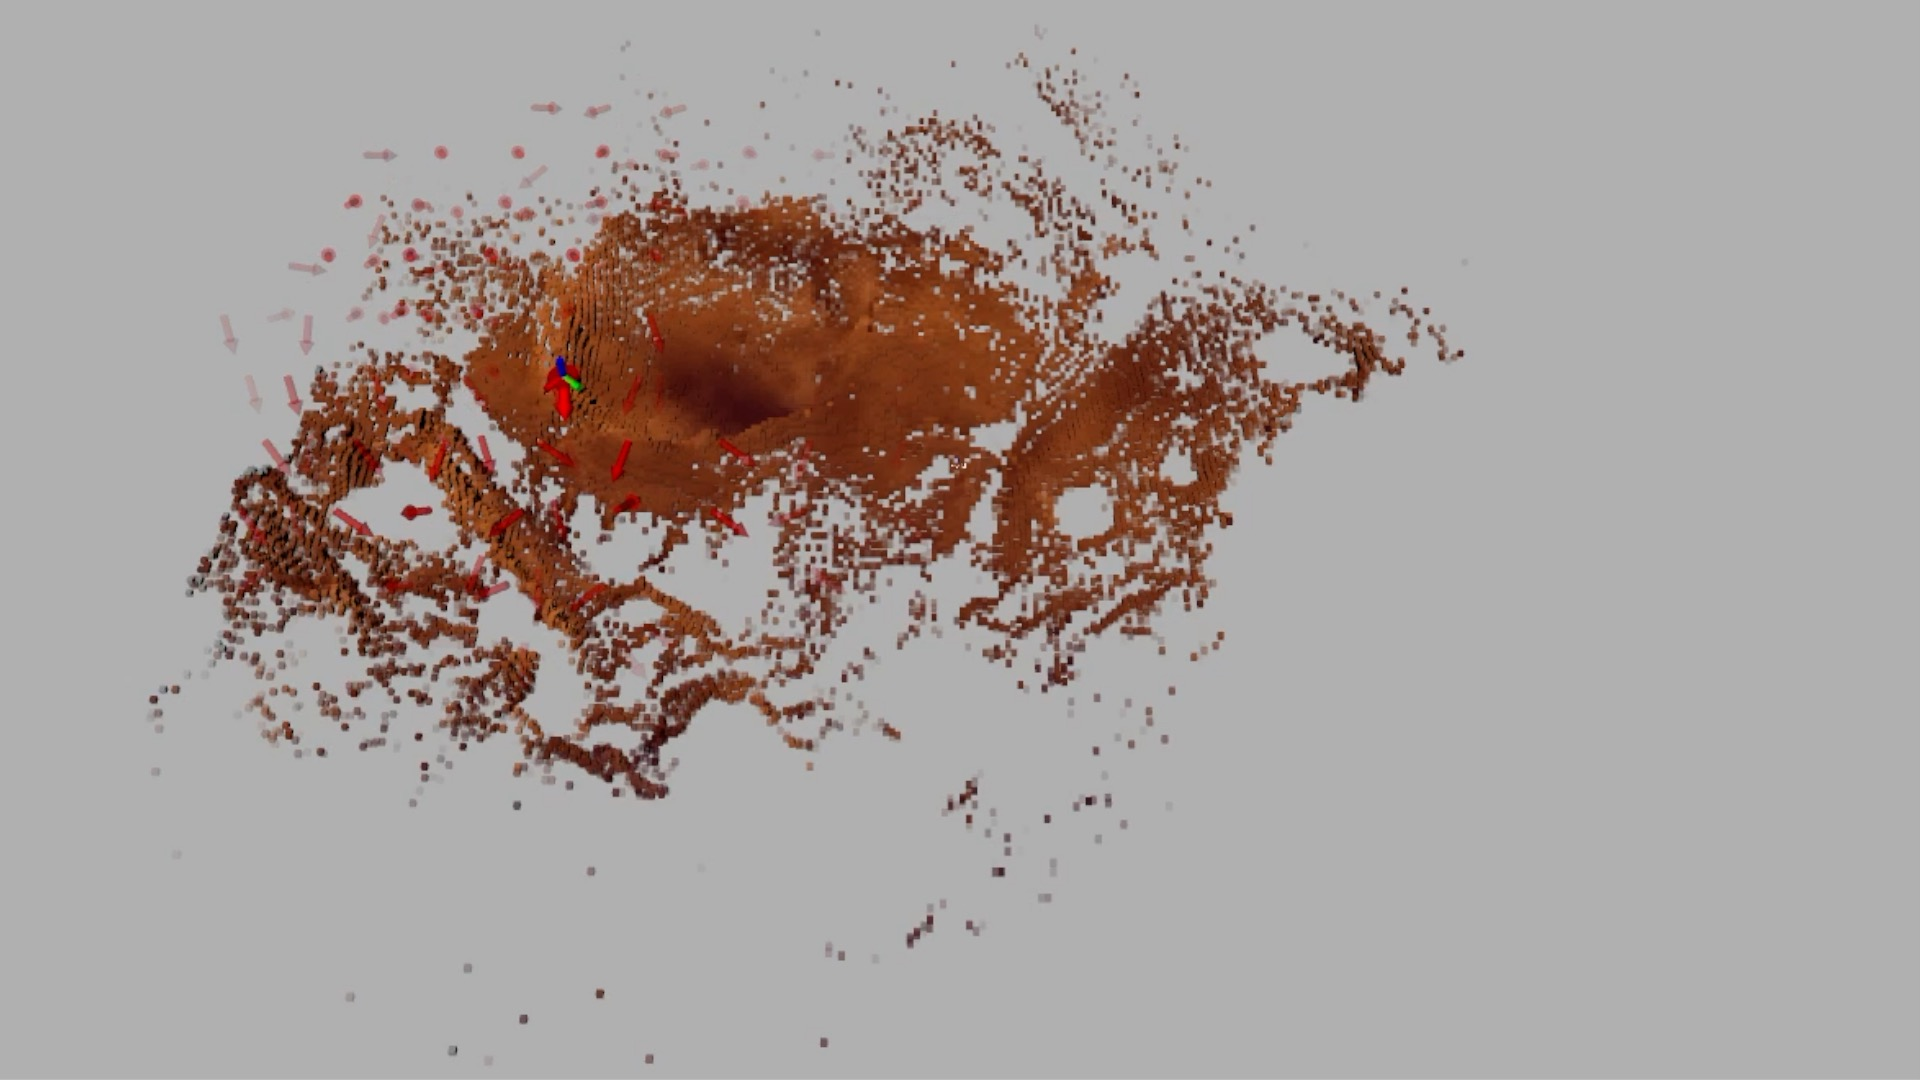
\includegraphics[height=0.5\textwidth]{FullMarsMap1min.jpg}
        		\caption{$1$ min}
		\vspace*{0.025\textwidth}
    	\end{subfigure}
	\centering
	\begin{subfigure}[t]{0.49\columnwidth}
           	\centering
          	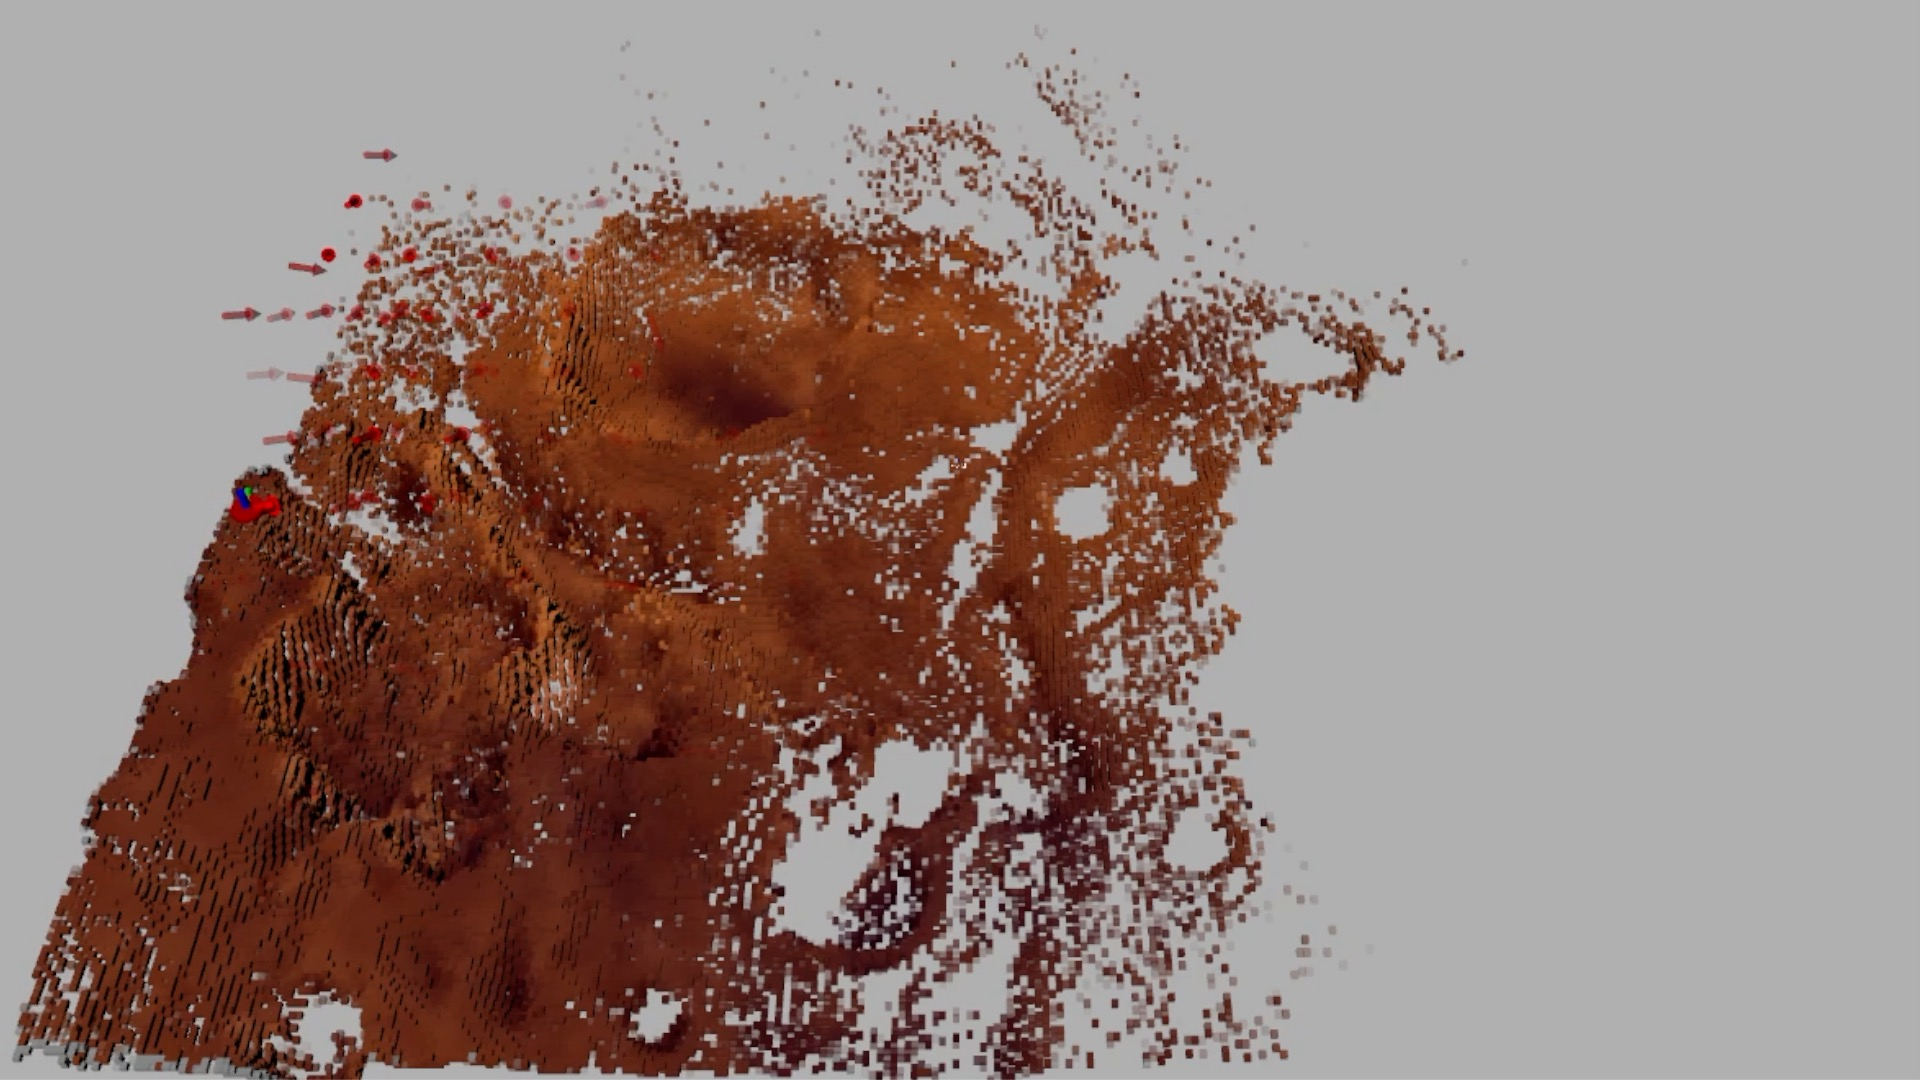
\includegraphics[height=0.5\textwidth]{FullMarsMap2min.jpg}
        		\caption{$2$ min}
		\vspace*{0.025\textwidth}
    	\end{subfigure}
    	\begin{subfigure}[t]{0.49\columnwidth}
           	\centering
          	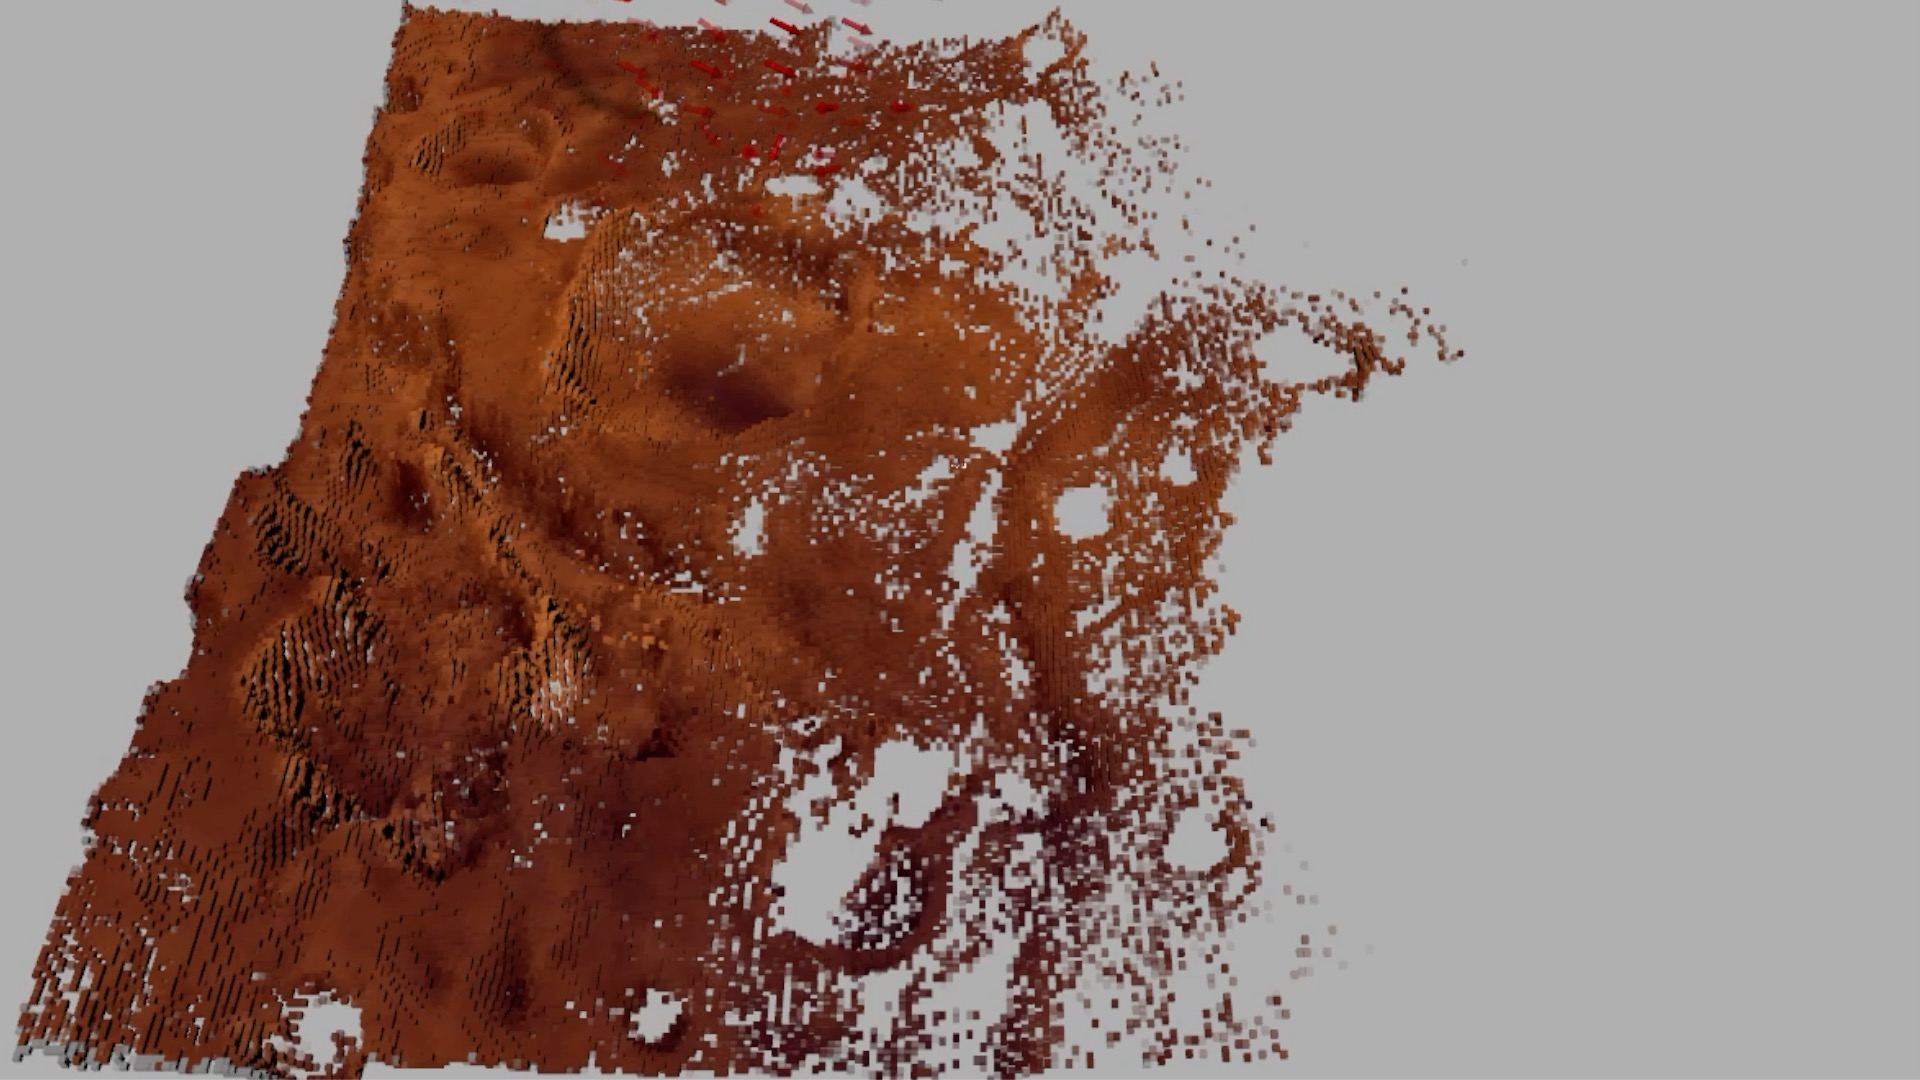
\includegraphics[height=0.5\textwidth]{FullMarsMap3min.jpg}
        		\caption{$3$ min}
		\vspace*{0.025\textwidth}
    	\end{subfigure}
	\centering
	\begin{subfigure}[t]{0.49\columnwidth}
           	\centering
          	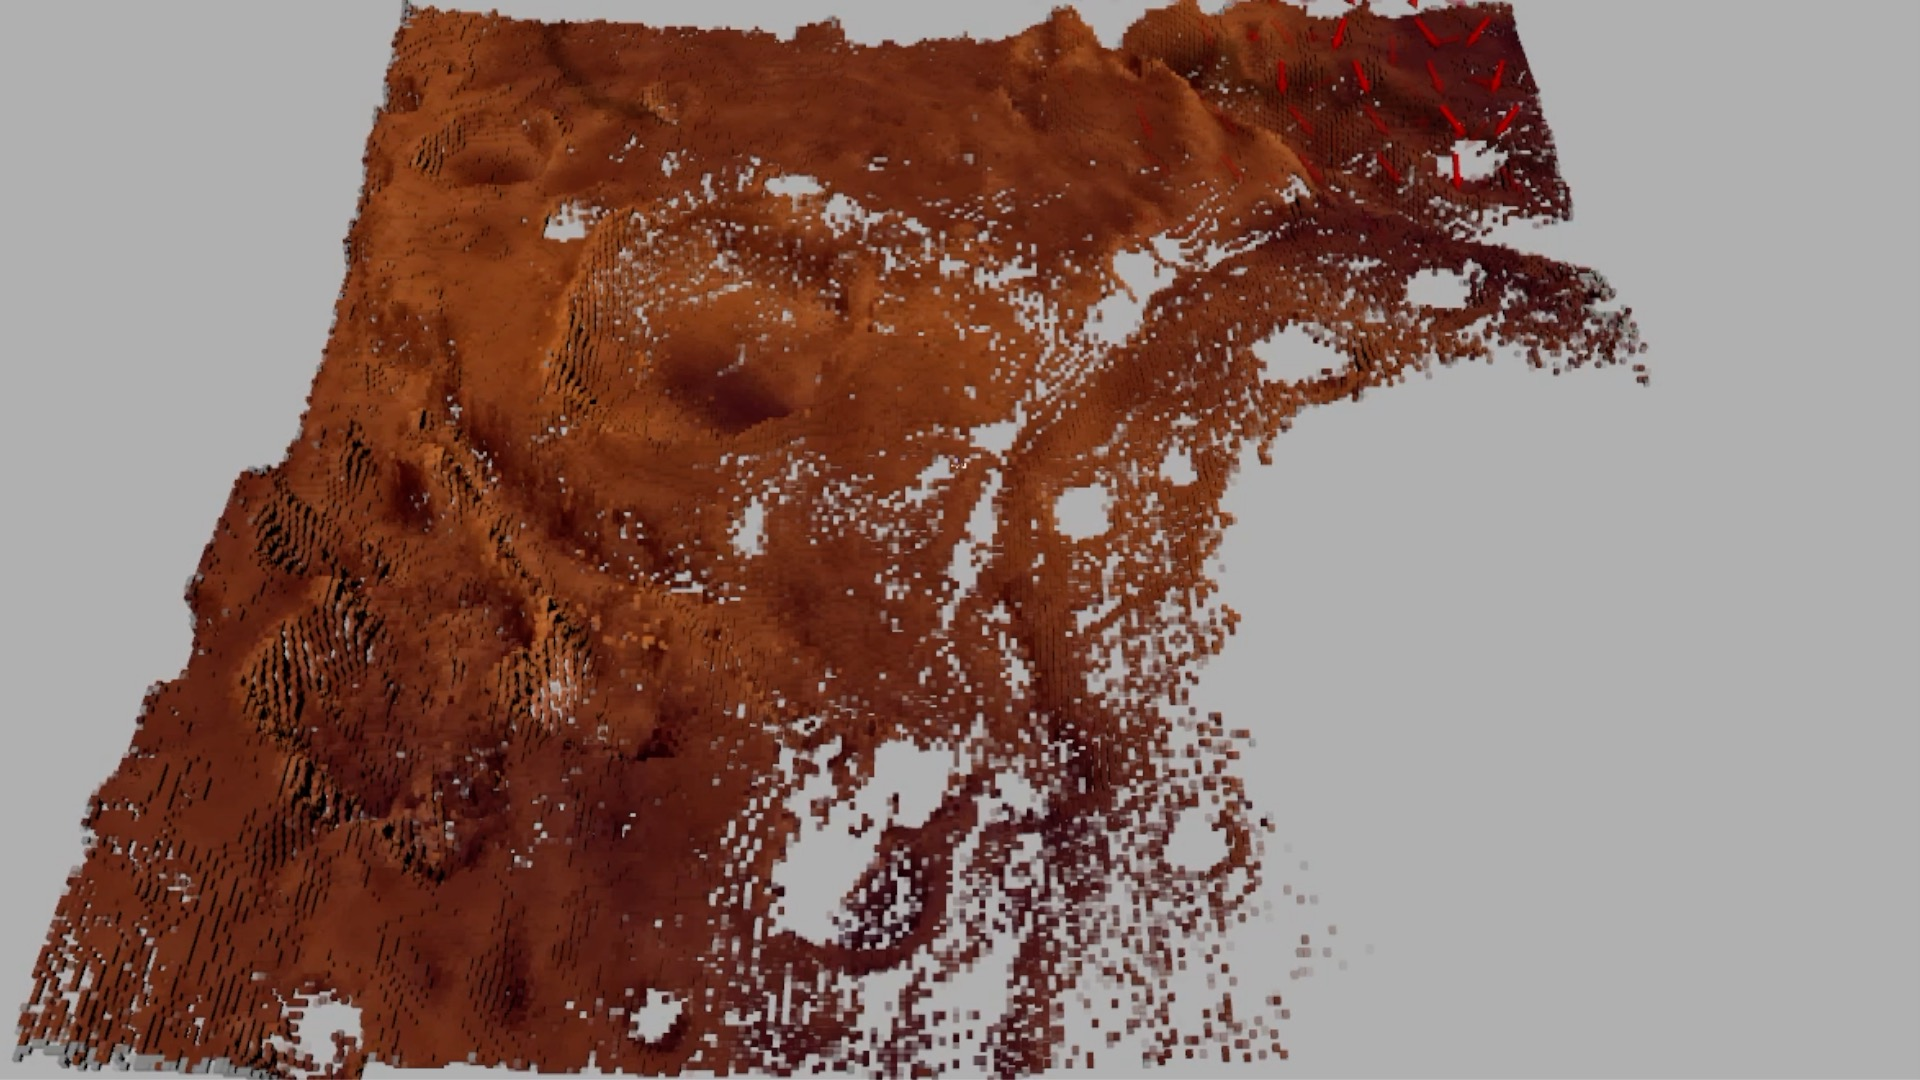
\includegraphics[height=0.5\textwidth]{FullMarsMap4min.jpg}
        		\caption{$4$ min}
		\vspace*{0.025\textwidth}
    	\end{subfigure}
    	\begin{subfigure}[t]{0.49\columnwidth}
           	\centering
          	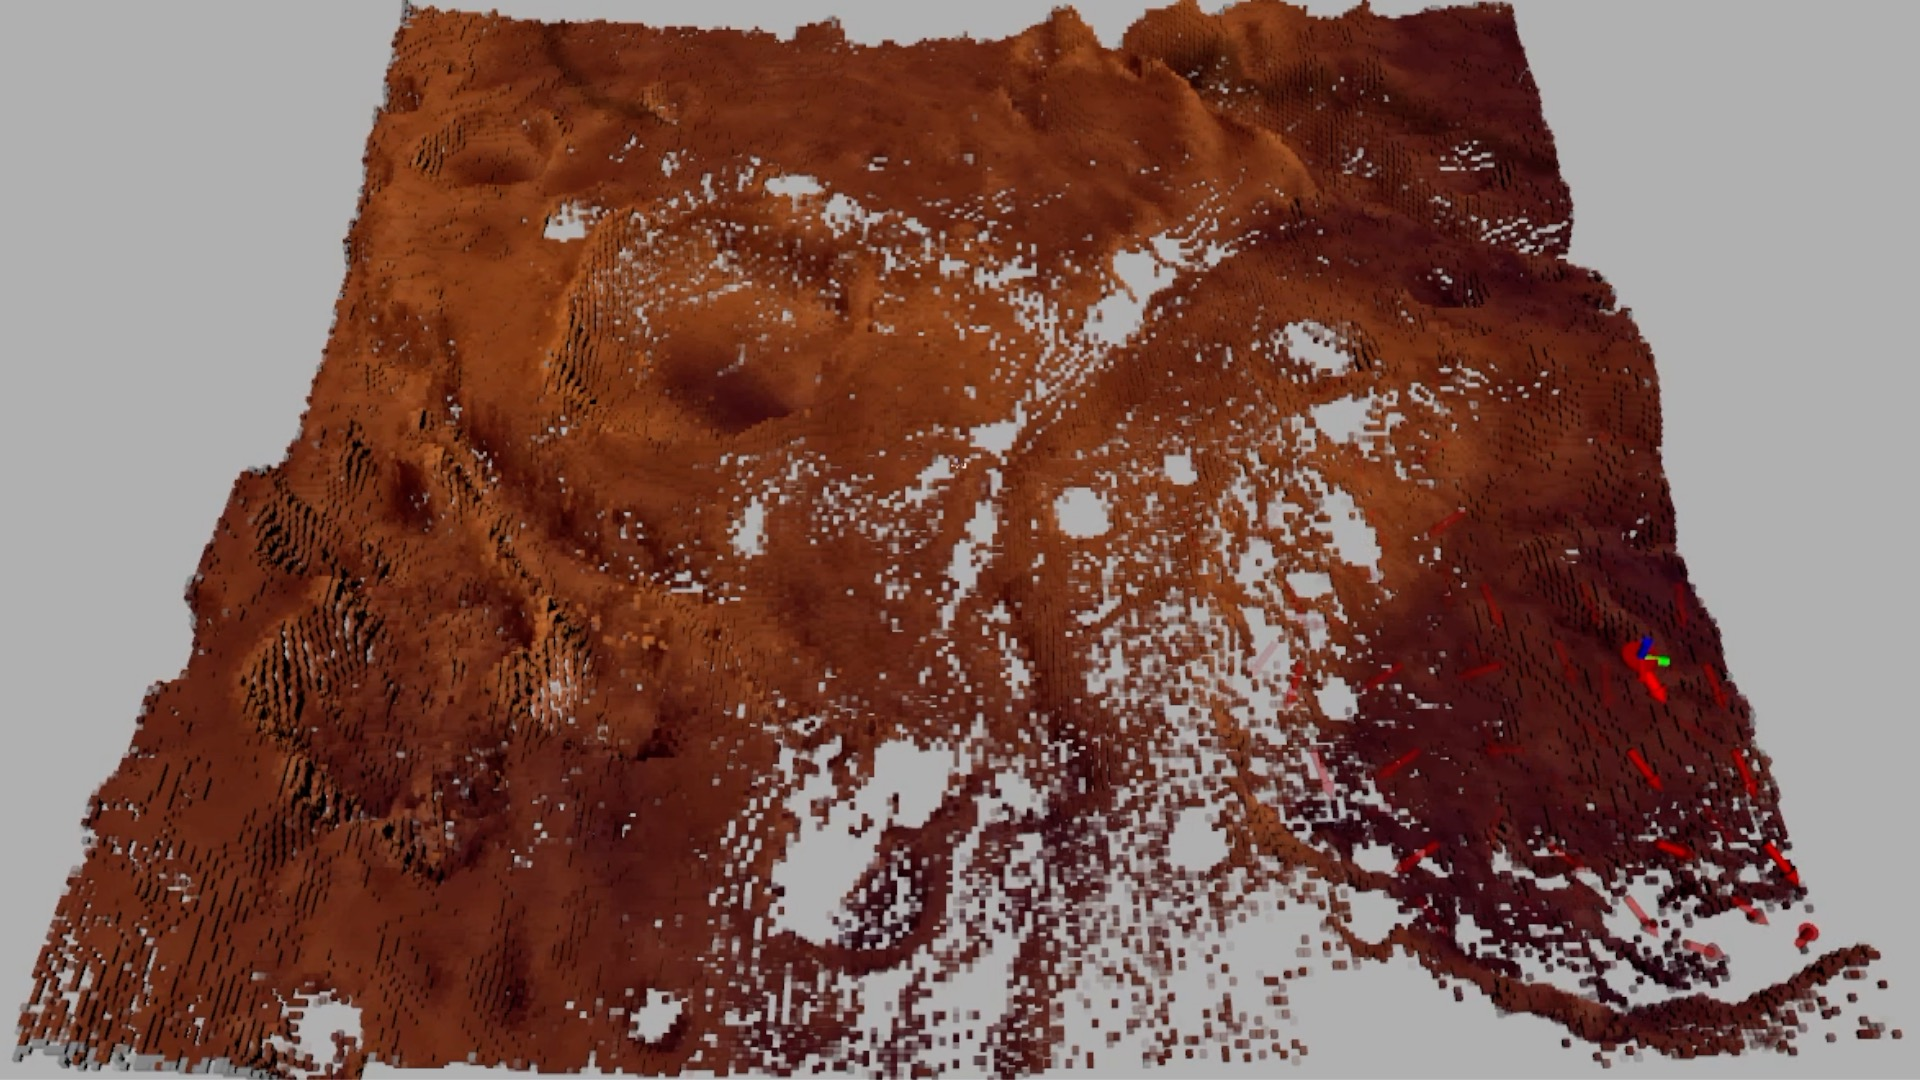
\includegraphics[height=0.5\textwidth]{FullMarsMap5min.jpg}
        		\caption{$5$ min}
		\vspace*{0.025\textwidth}
    	\end{subfigure}
	\centering
	\begin{subfigure}[t]{0.49\columnwidth}
           	\centering
          	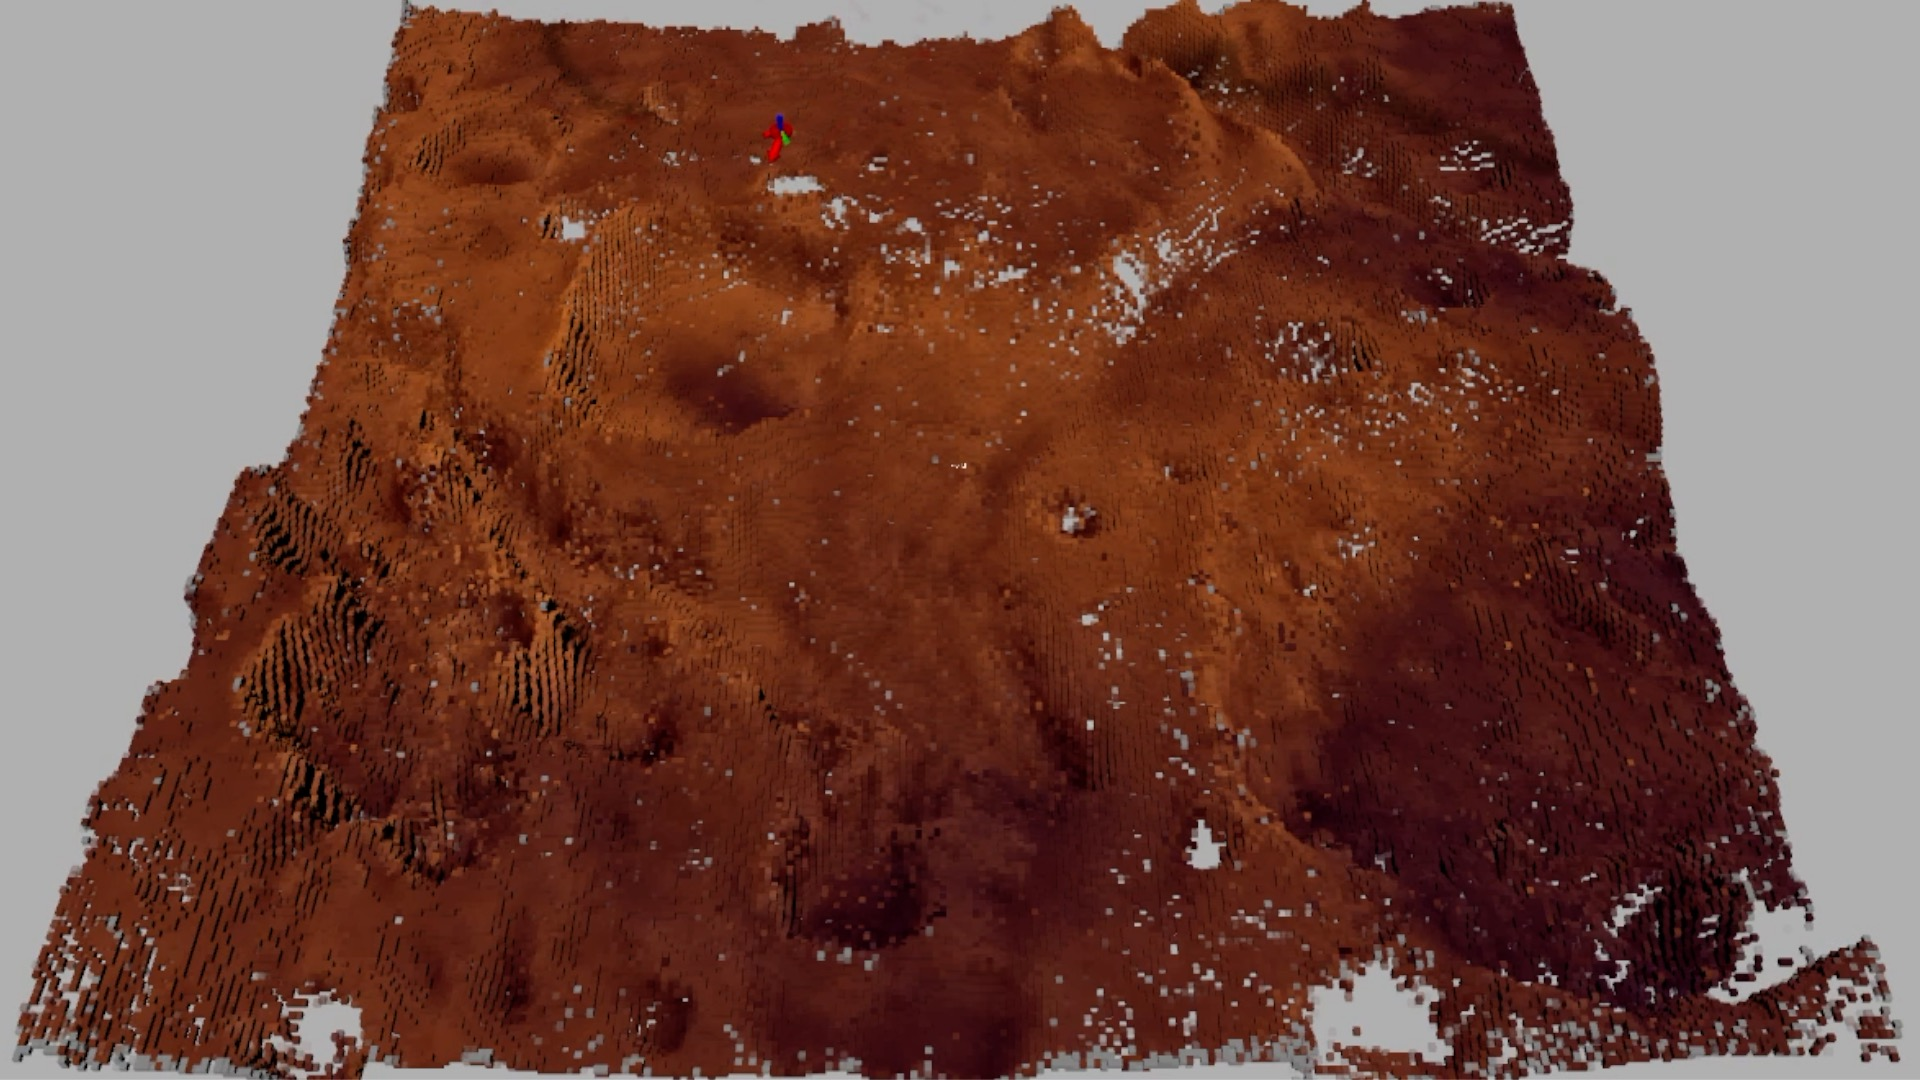
\includegraphics[height=0.5\textwidth]{FullMarsMap10min.jpg}
        		\caption{$10$ min}
		\vspace*{0.025\textwidth}
    	\end{subfigure}
    	\begin{subfigure}[t]{0.49\columnwidth}
           	\centering
          	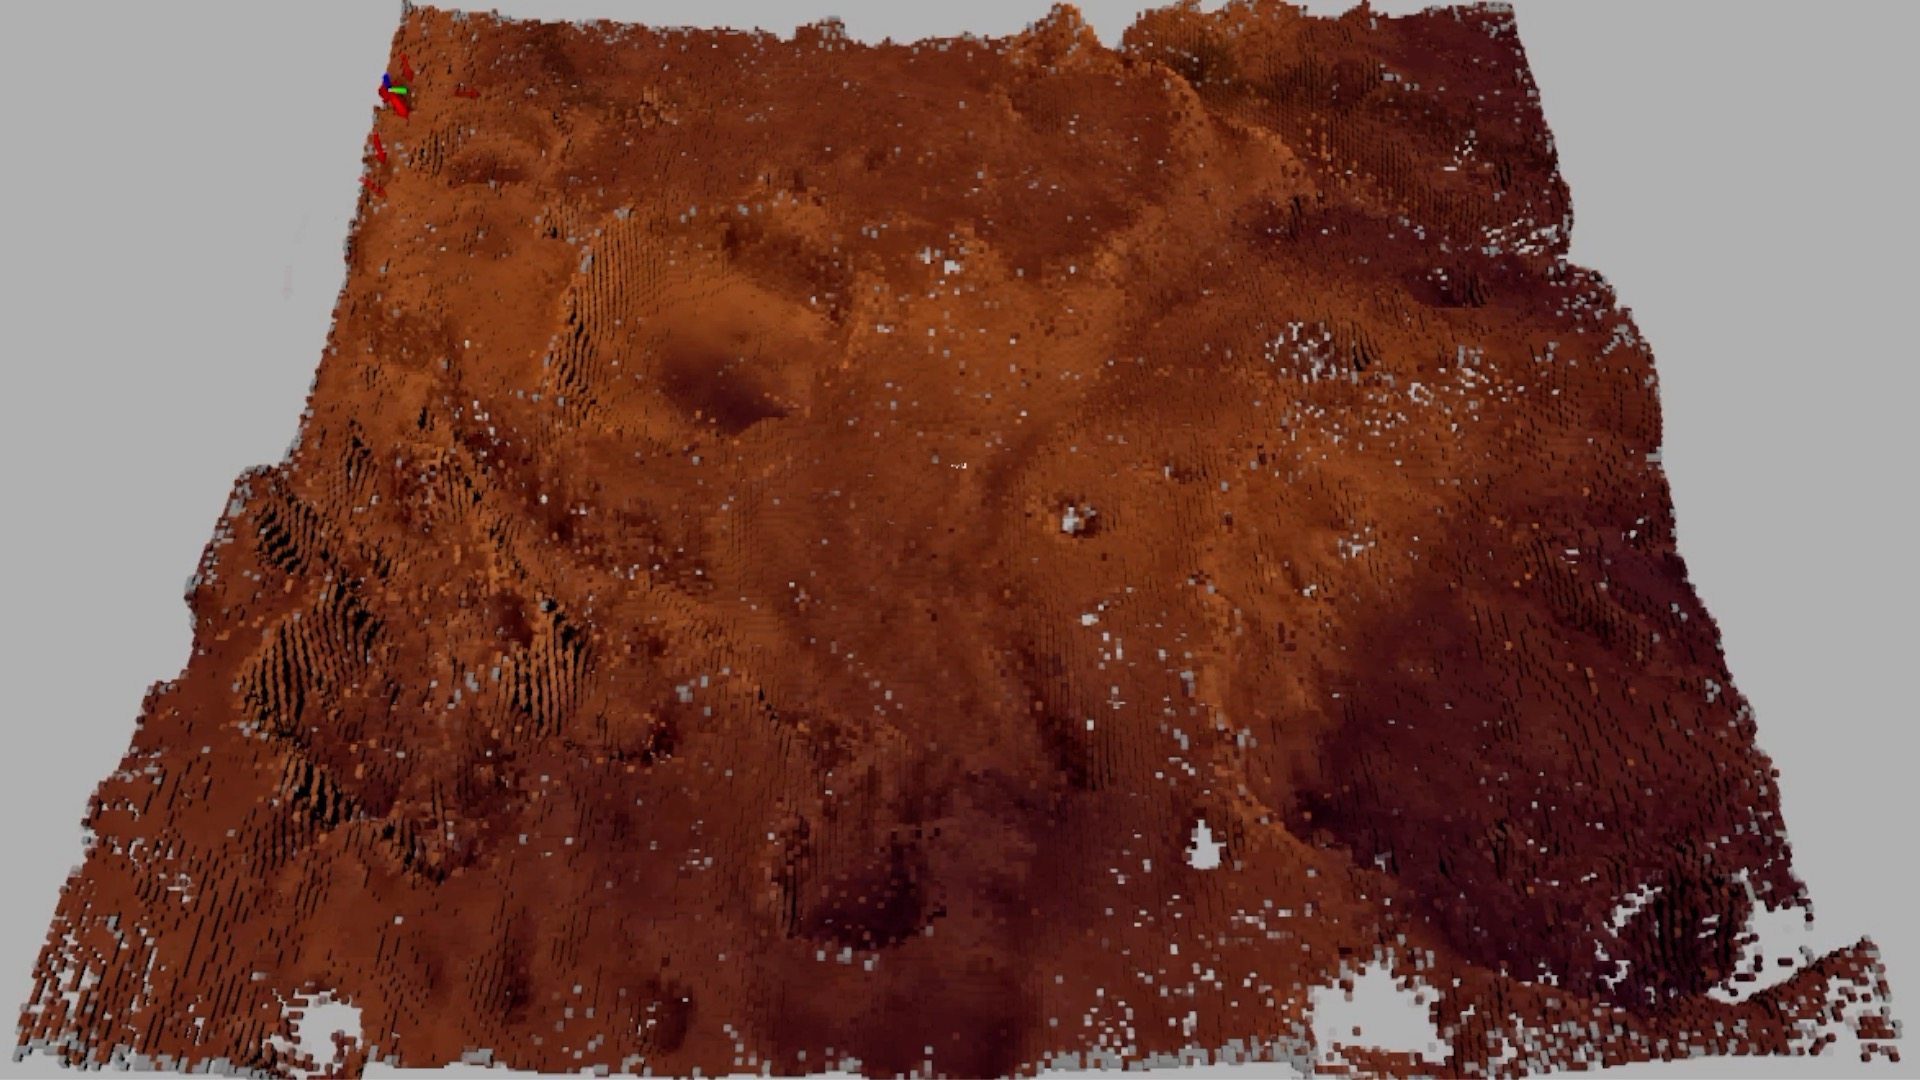
\includegraphics[height=0.5\textwidth]{FullMarsMap15min.jpg}
        		\caption{$15$ min}
		\vspace*{0.025\textwidth}
    	\end{subfigure}
\caption{In Case 1, the robot (red disk with arrow indicating laser direction) moves toward candidate poses (red arrows, more opaque for greater reward) based on expected entropy change of the 3D probabilistic occupancy grid map $m$ (cubes: greater opacity for greater occupancy probability) of the surface of Mars.}
\label{fig:mars3DogmCase1}
\end{figure}


\begin{figure}[!t]
	\centering
	\begin{subfigure}[t]{0.49\columnwidth}
           	\centering
          	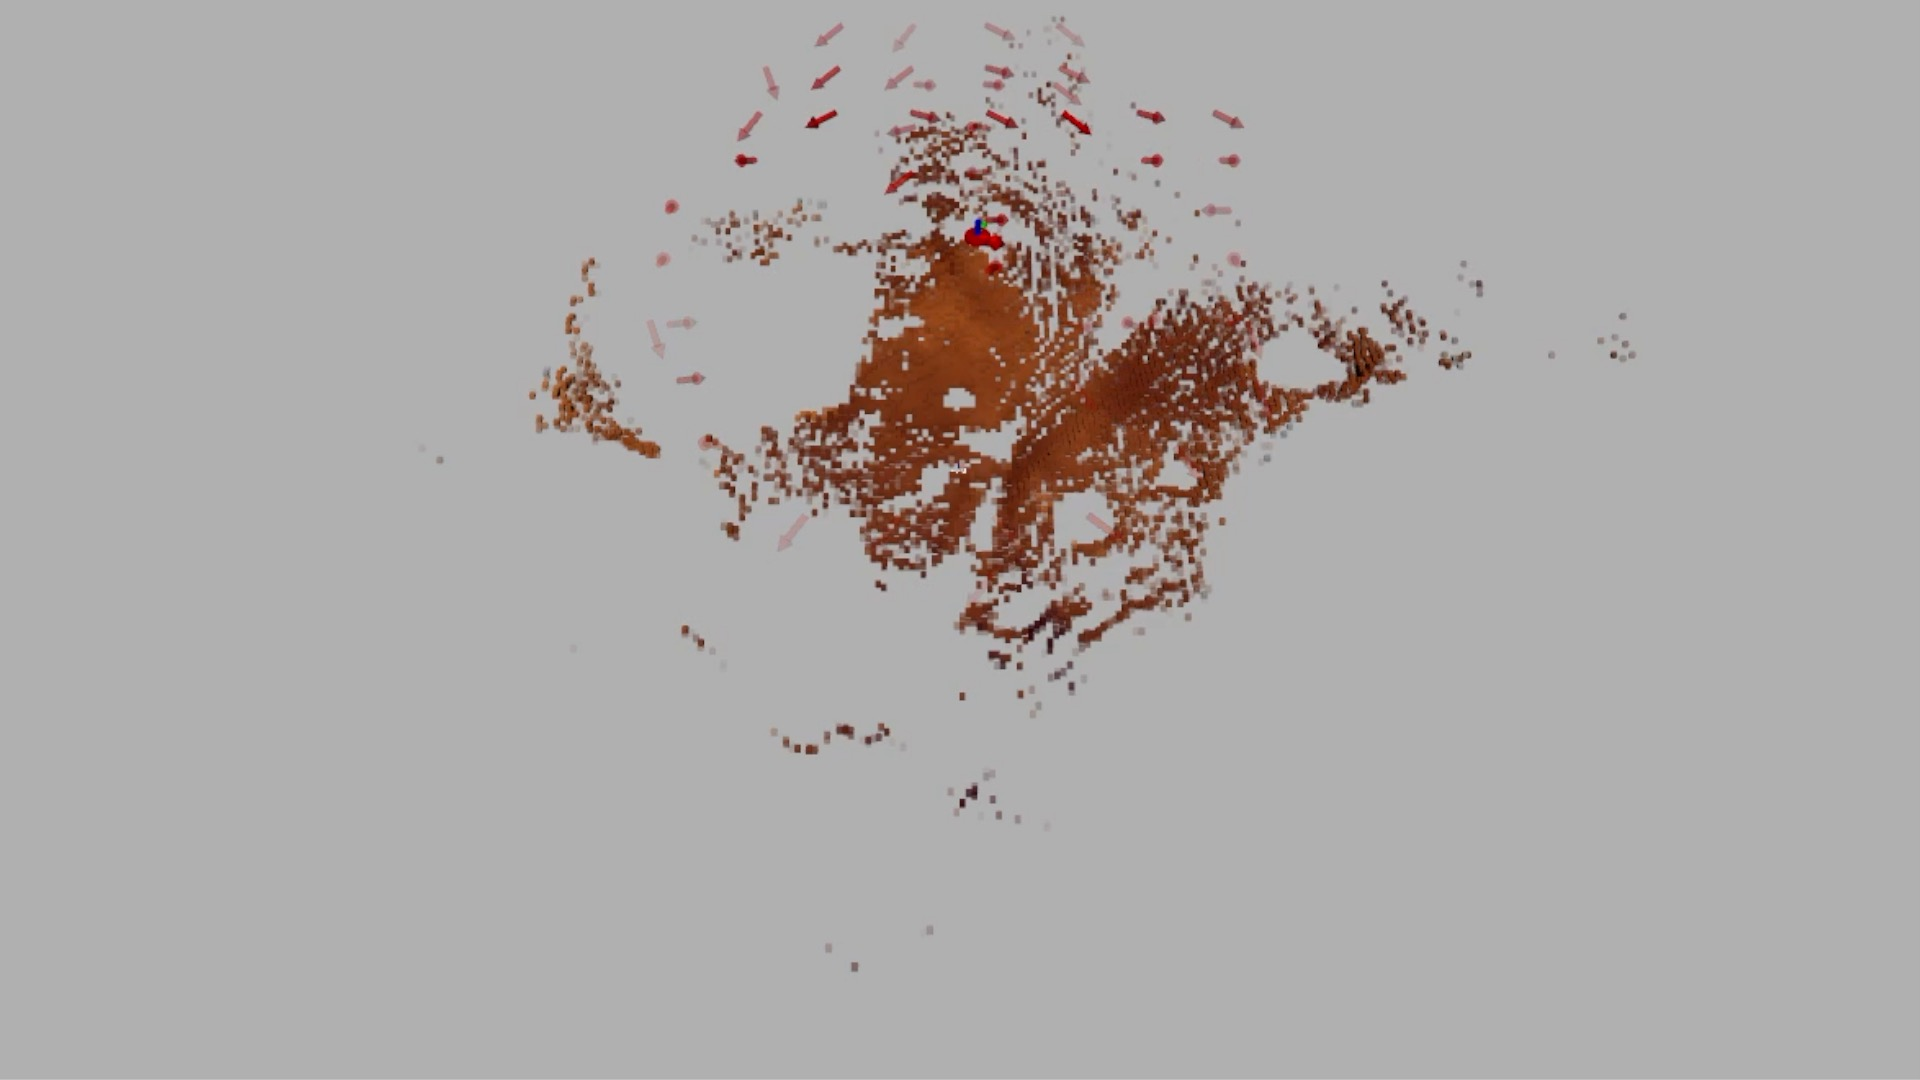
\includegraphics[height=0.5\textwidth]{RdcdMarsMap30sec.jpg}
        		\caption{$30$ sec}
		\vspace*{0.025\textwidth}
    	\end{subfigure}
    	\begin{subfigure}[t]{0.49\columnwidth}
           	\centering
          	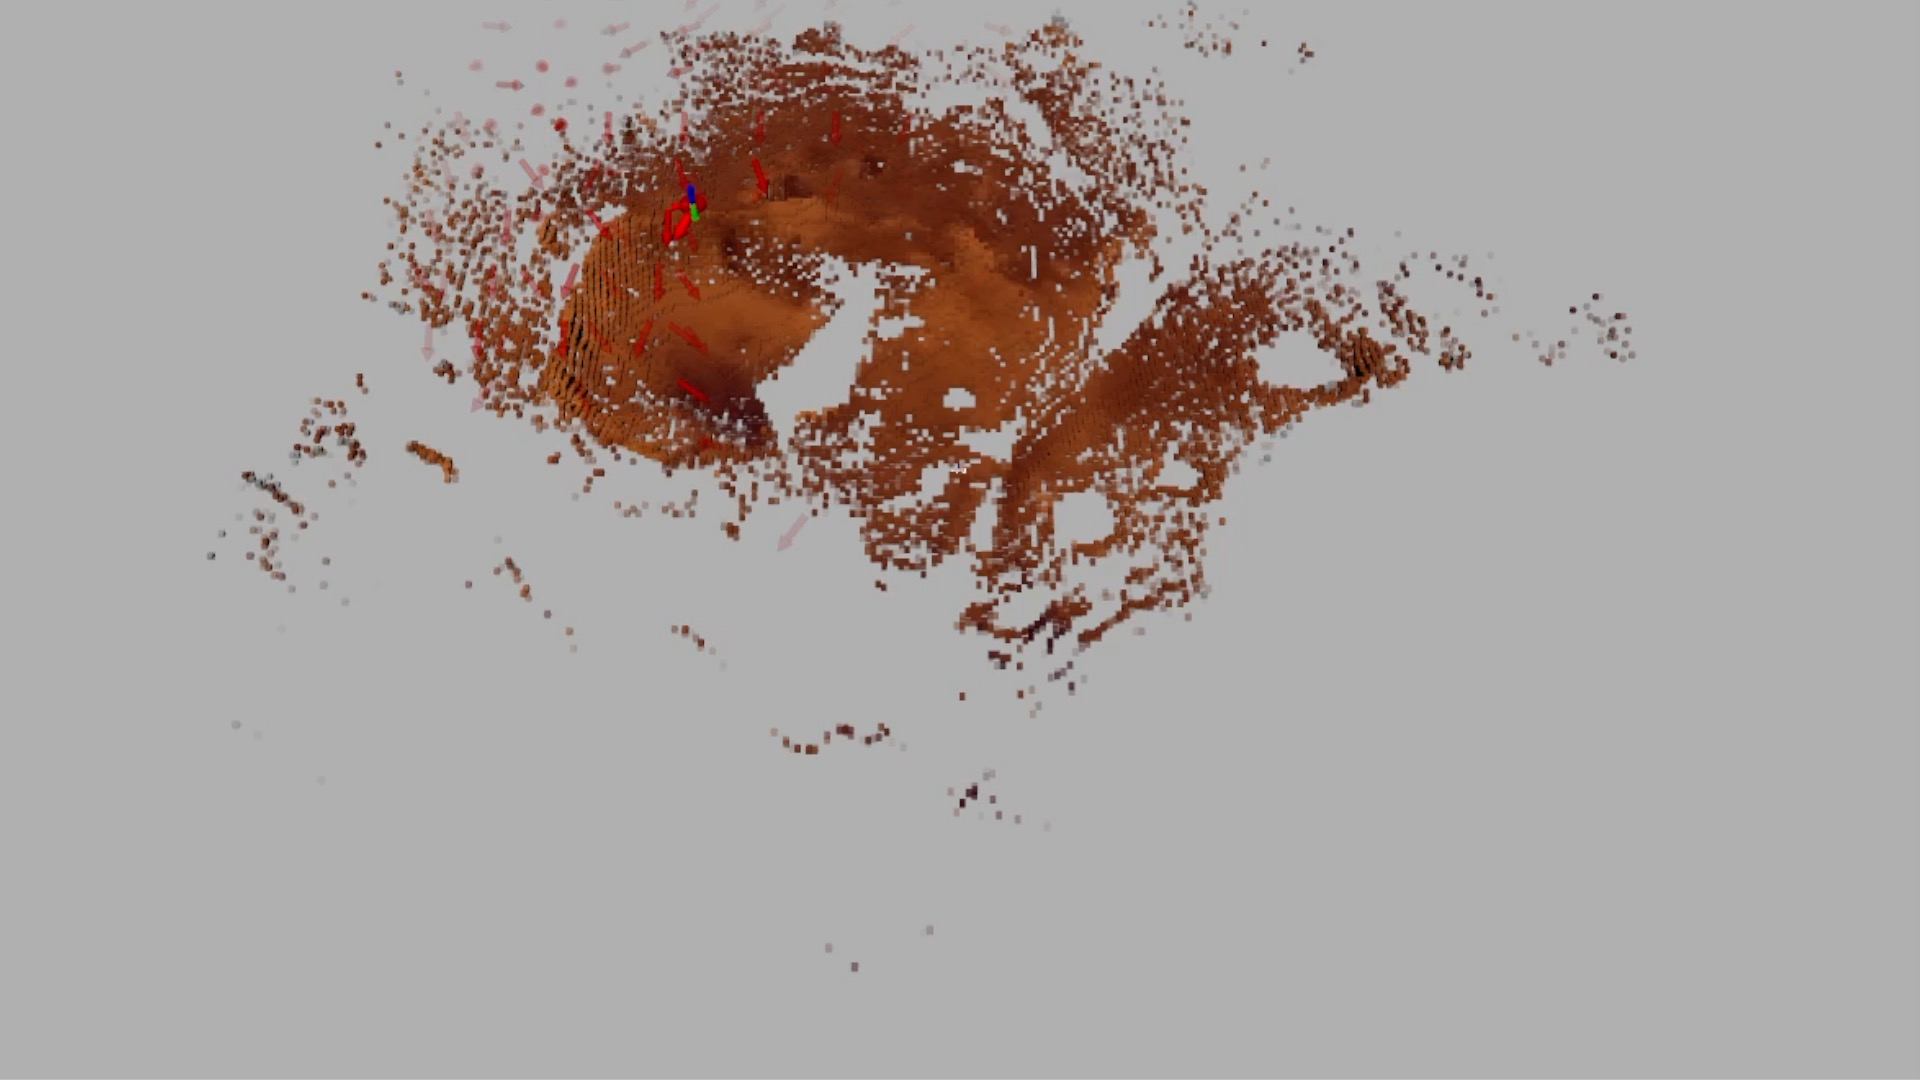
\includegraphics[height=0.5\textwidth]{RdcdMarsMap1min.jpg}
        		\caption{$1$ min}
		\vspace*{0.025\textwidth}
    	\end{subfigure}
	\centering
	\begin{subfigure}[t]{0.49\columnwidth}
           	\centering
          	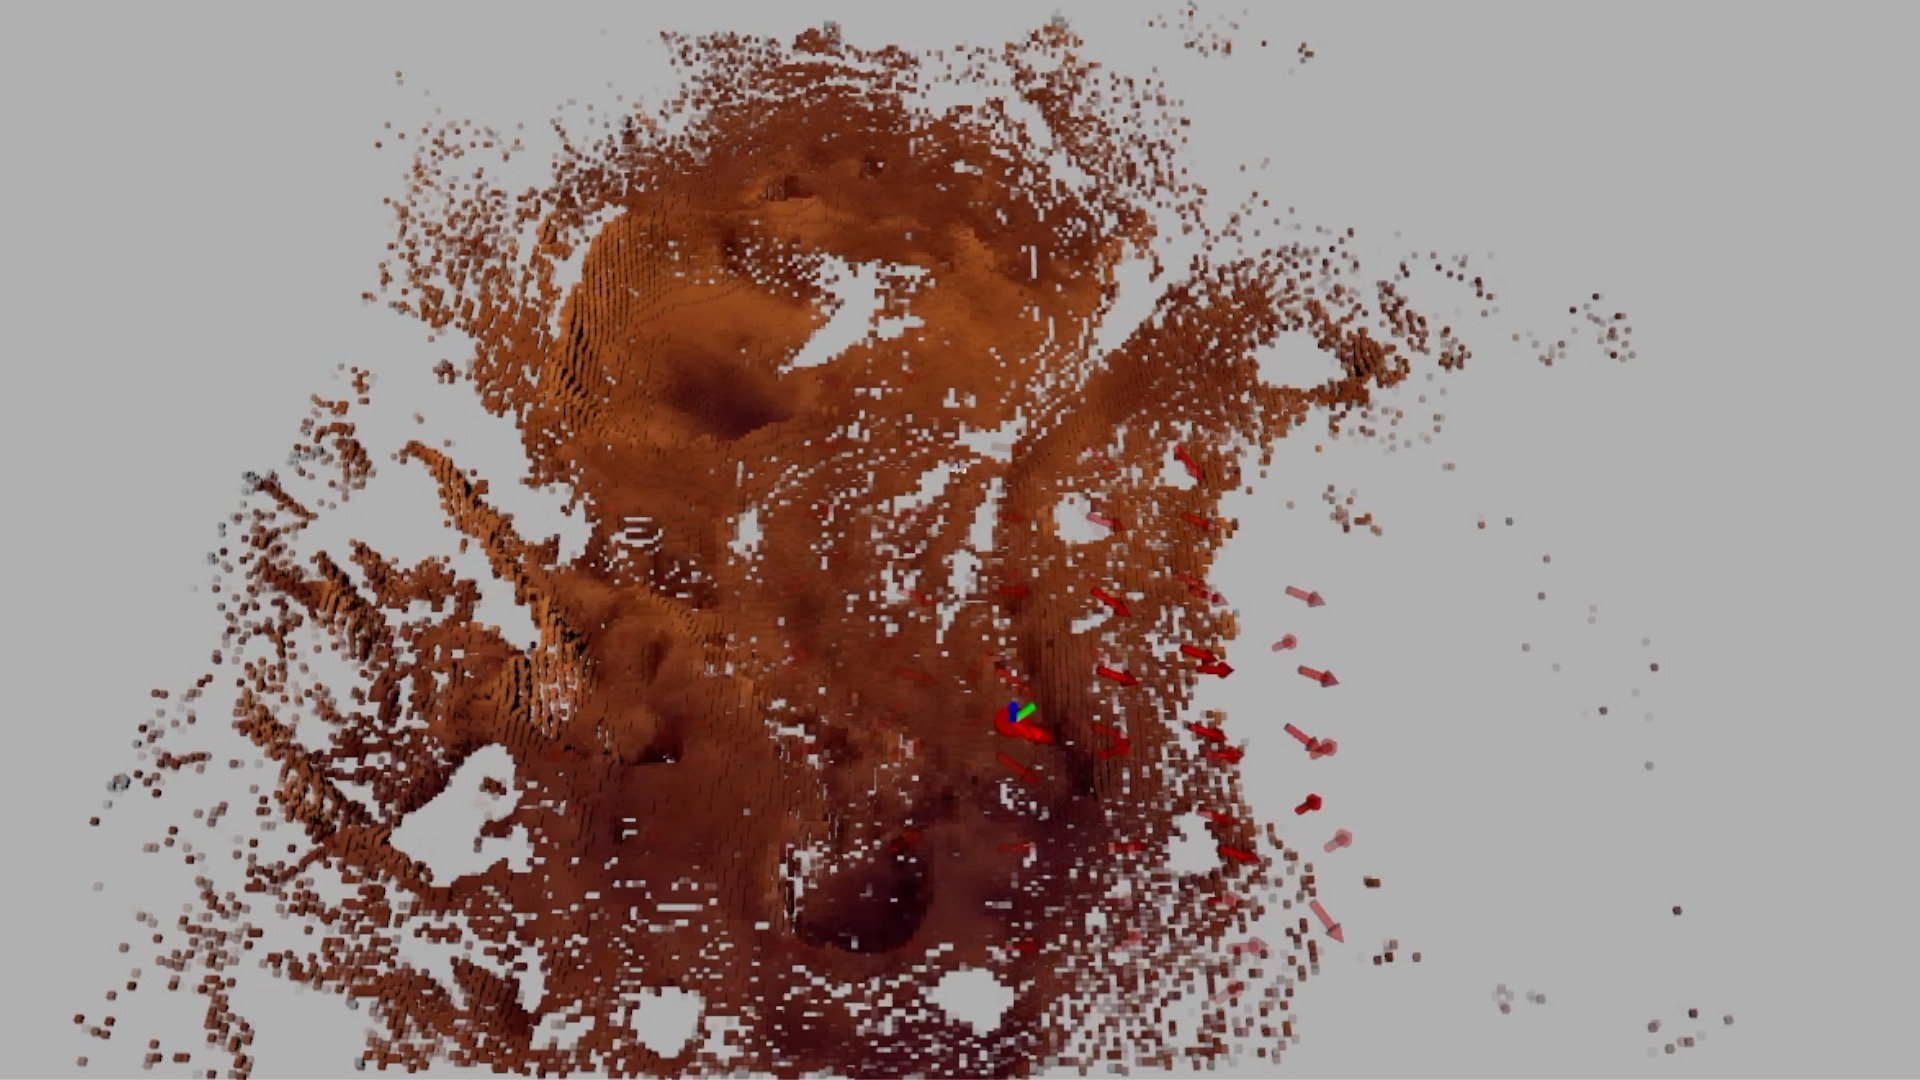
\includegraphics[height=0.5\textwidth]{RdcdMarsMap2min.jpg}
        		\caption{$2$ min}
		\vspace*{0.025\textwidth}
    	\end{subfigure}
    	\begin{subfigure}[t]{0.49\columnwidth}
           	\centering
          	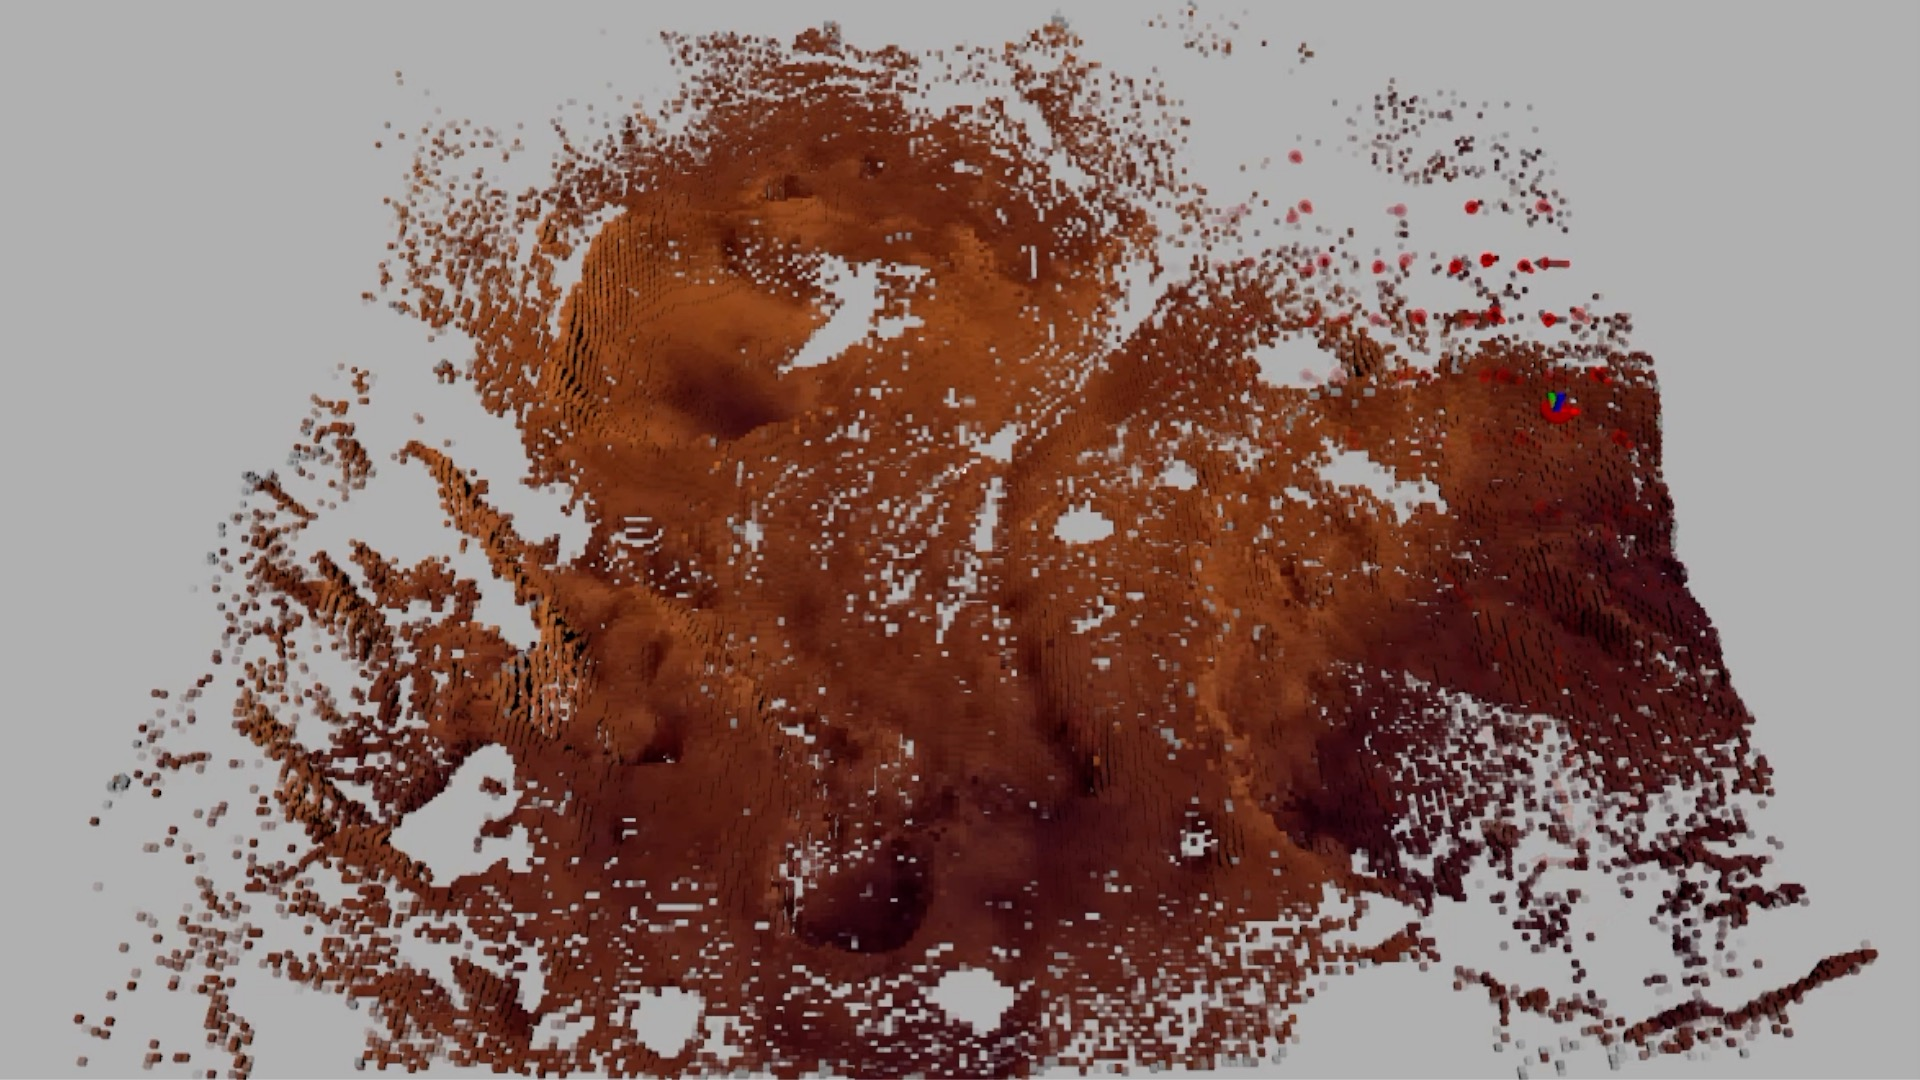
\includegraphics[height=0.5\textwidth]{RdcdMarsMap3min.jpg}
        		\caption{$3$ min}
		\vspace*{0.025\textwidth}
    	\end{subfigure}
	\centering
	\begin{subfigure}[t]{0.49\columnwidth}
           	\centering
          	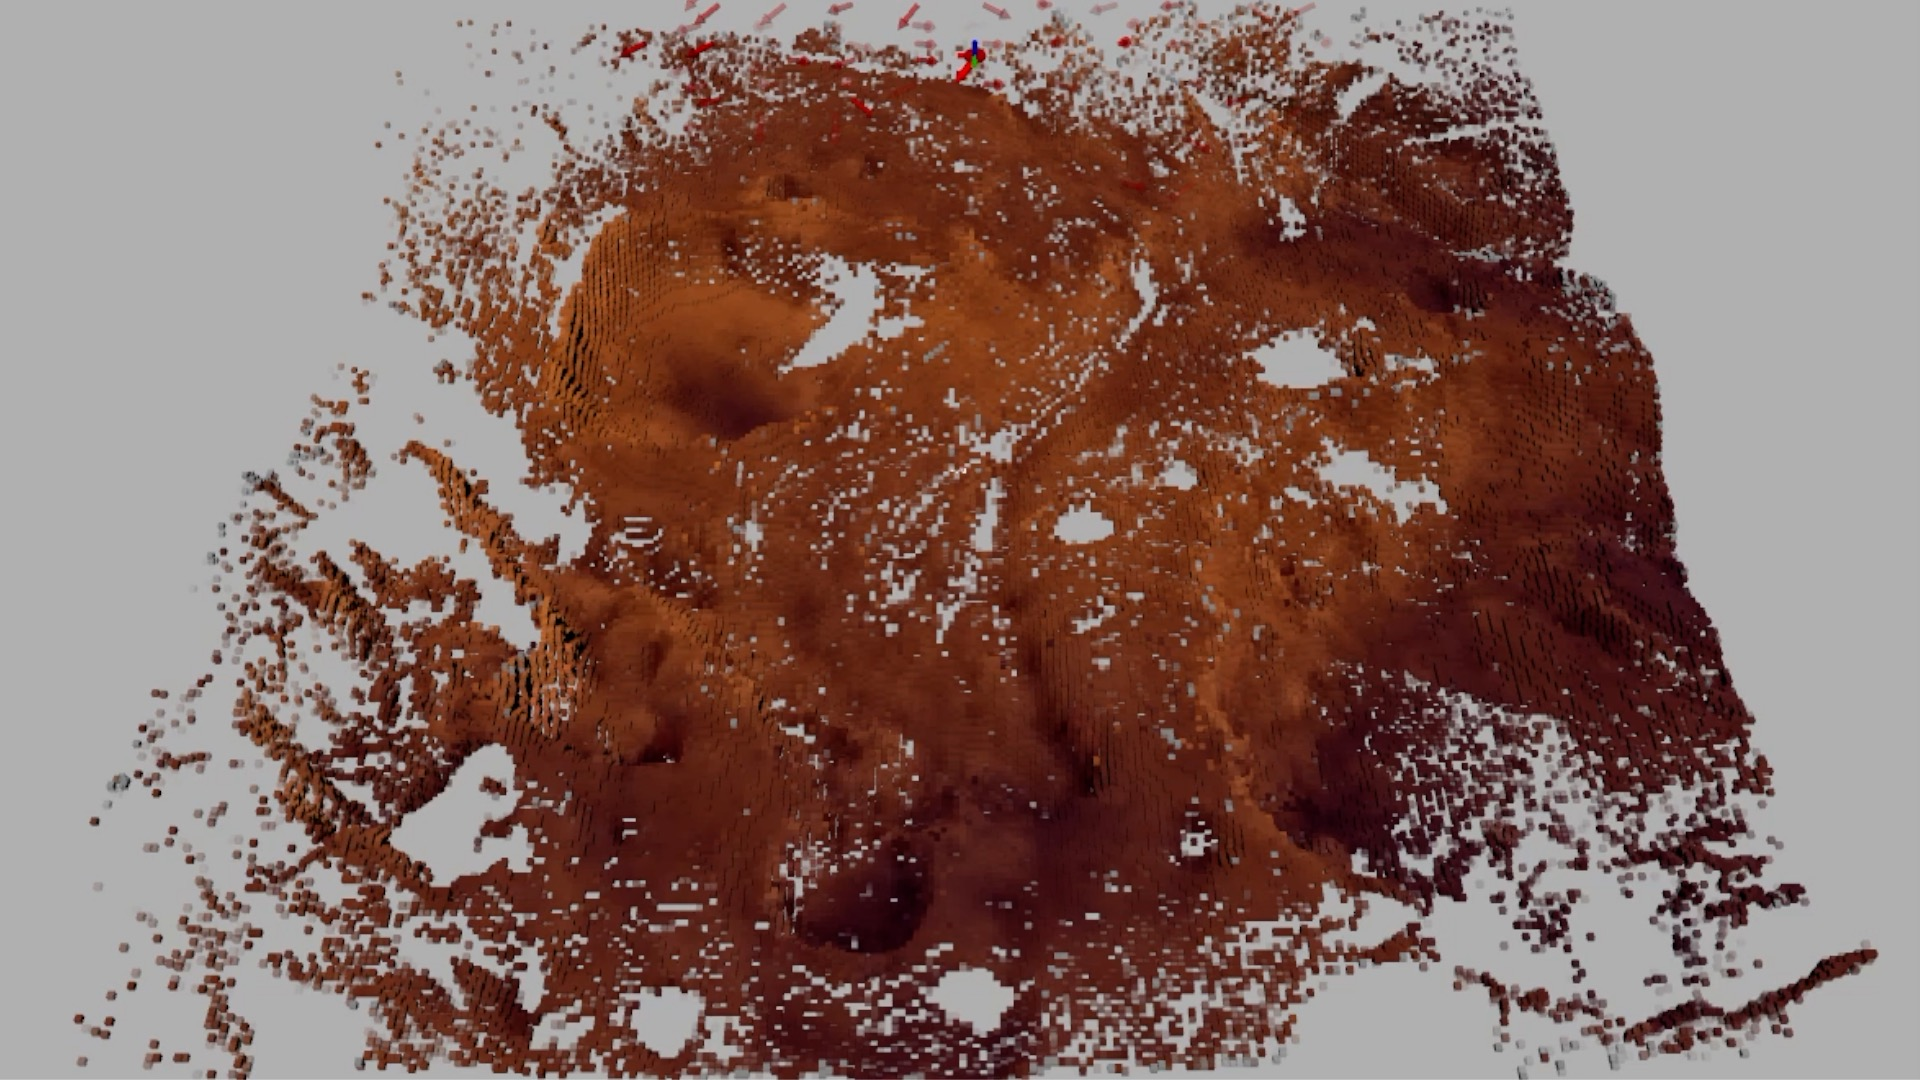
\includegraphics[height=0.5\textwidth]{RdcdMarsMap4min.jpg}
        		\caption{$4$ min}
		\vspace*{0.025\textwidth}
    	\end{subfigure}
    	\begin{subfigure}[t]{0.49\columnwidth}
           	\centering
          	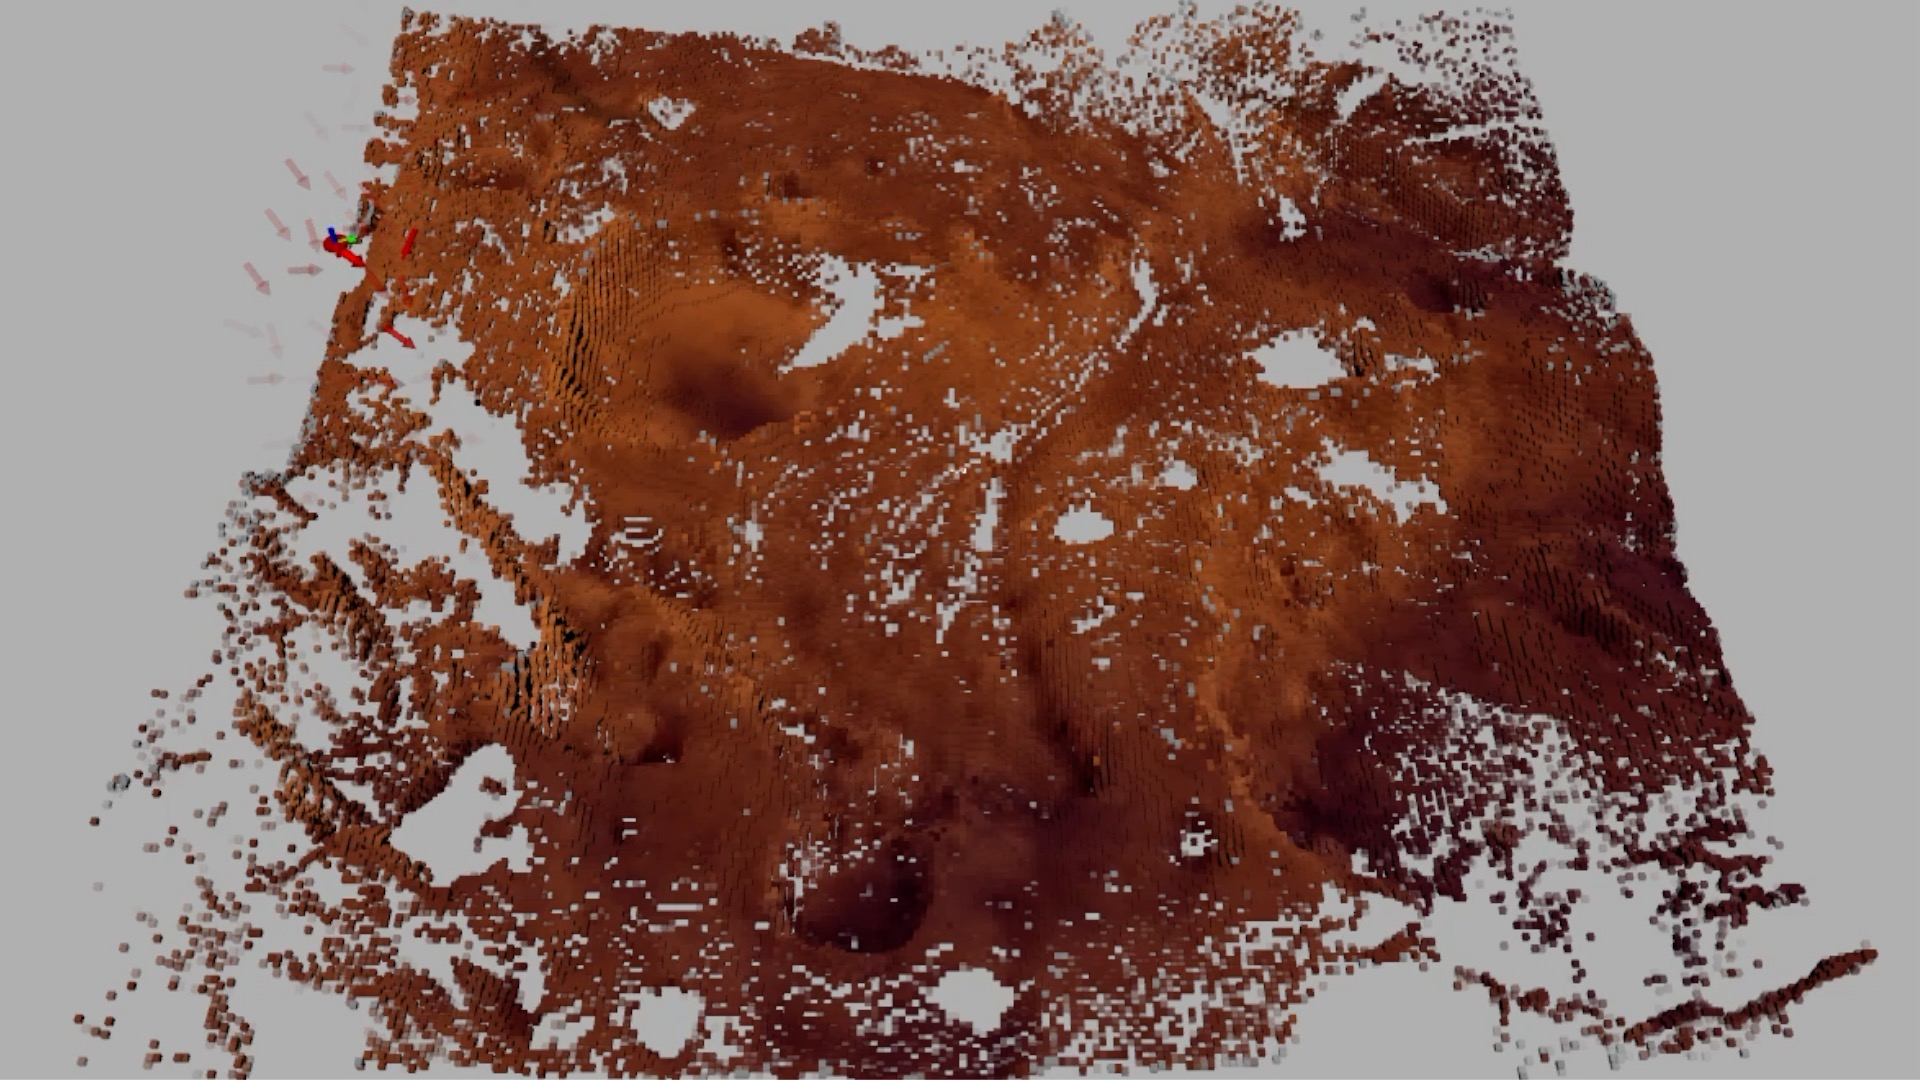
\includegraphics[height=0.5\textwidth]{RdcdMarsMap5min.jpg}
        		\caption{$5$ min}
		\vspace*{0.025\textwidth}
    	\end{subfigure}
	\centering
	\begin{subfigure}[t]{0.49\columnwidth}
           	\centering
          	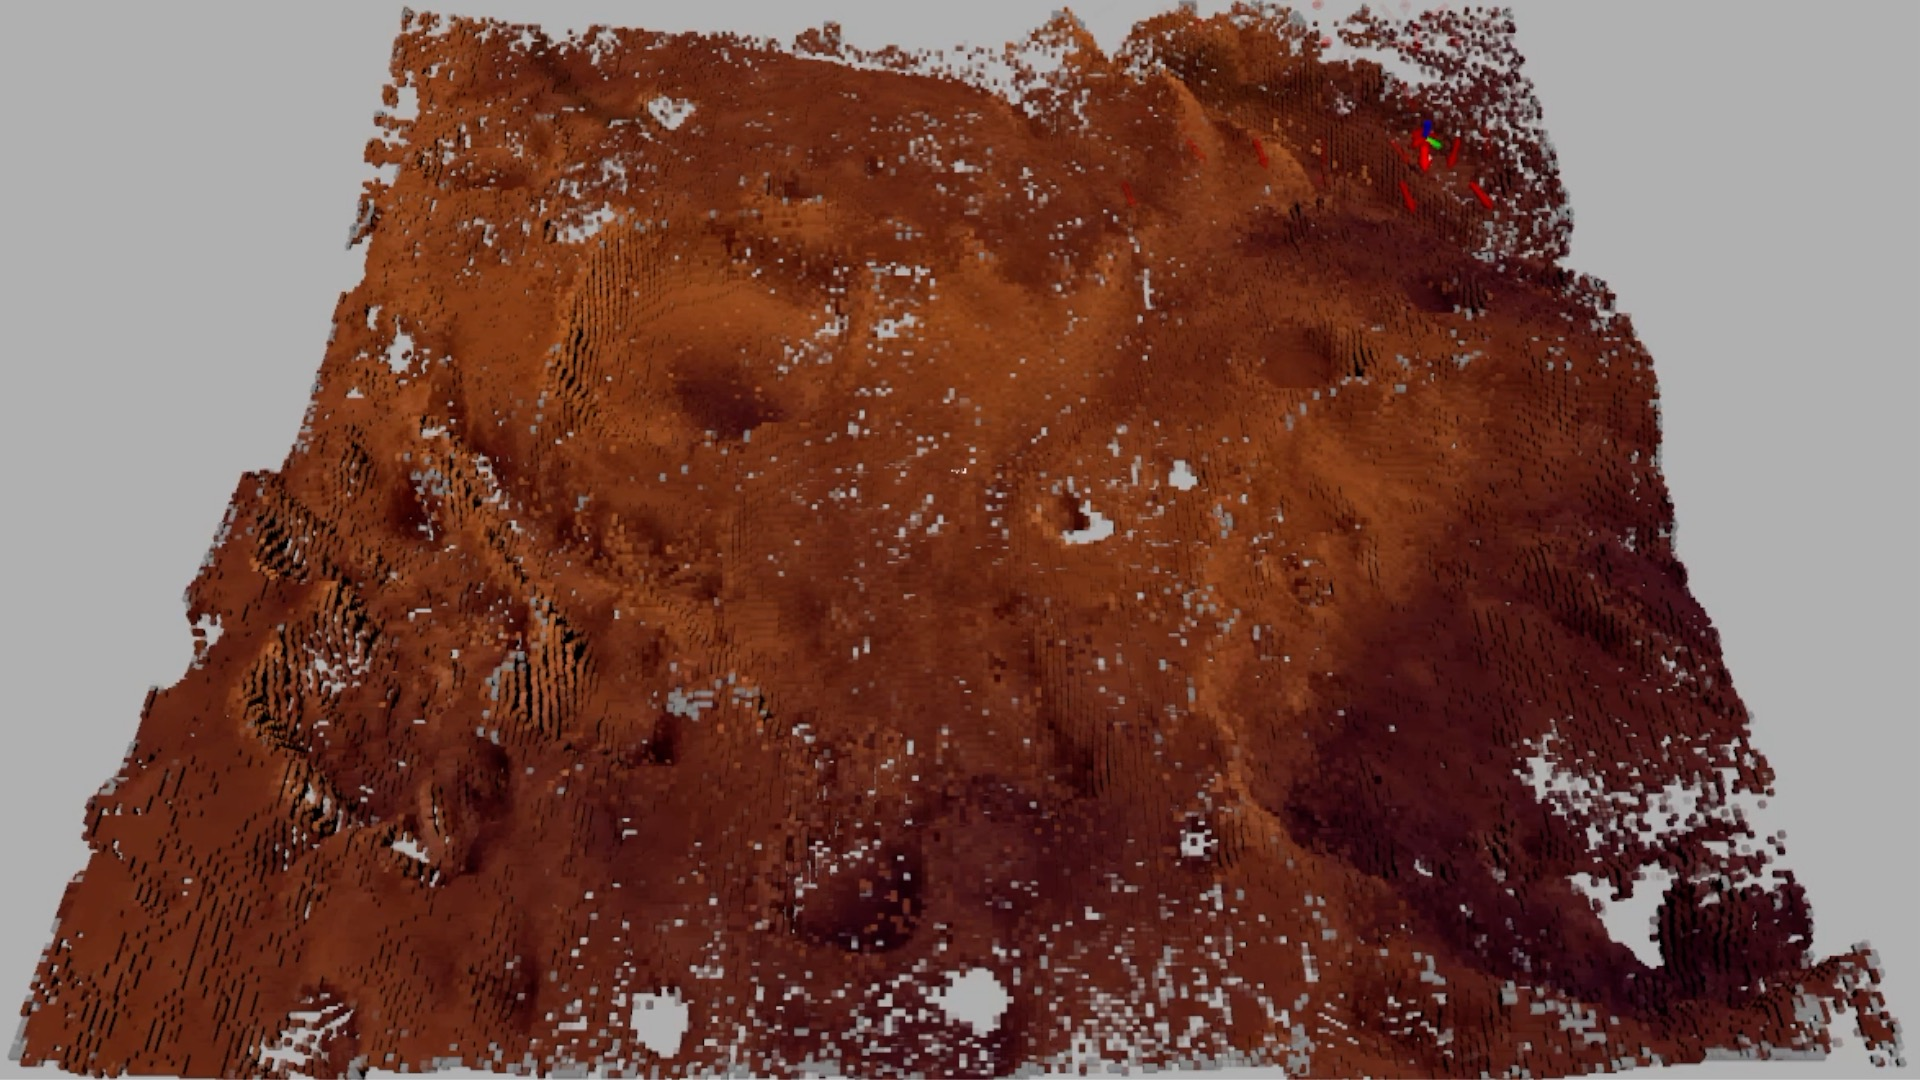
\includegraphics[height=0.5\textwidth]{RdcdMarsMap10min.jpg}
        		\caption{$10$ min}
		\vspace*{0.025\textwidth}
    	\end{subfigure}
    	\begin{subfigure}[t]{0.49\columnwidth}
           	\centering
          	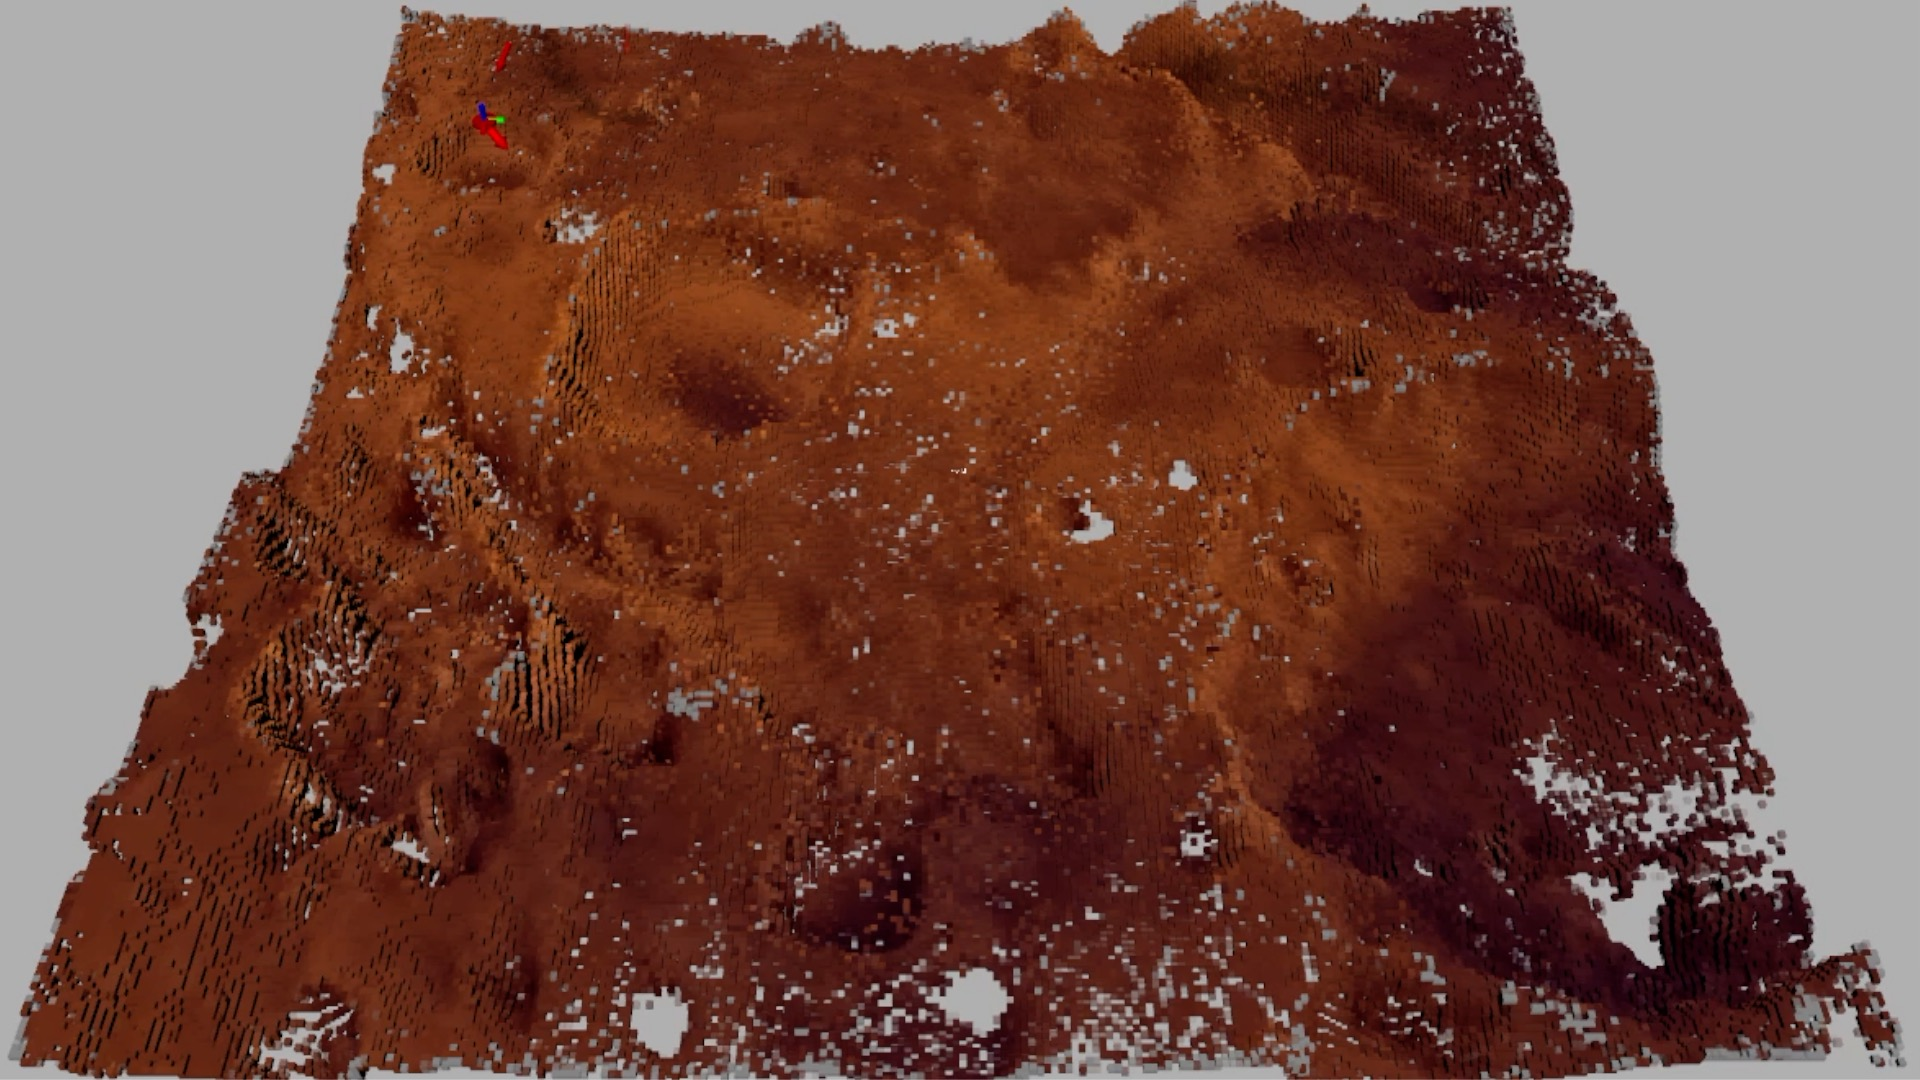
\includegraphics[height=0.5\textwidth]{RdcdMarsMap15min.jpg}
        		\caption{$15$ min}
		\vspace*{0.025\textwidth}
    	\end{subfigure}
\caption{In Case 2, the robot (red disk with arrow indicating laser direction) generates a 3D probabilistic occupancy grid map $m$ (cubes: greater opacity for greater occupancy probability), which is used to generate a reduced map $m_\text{reduced}$ based on \refeqn{Proj3DMapComb}. The robot moves toward candidate poses (red arrows, more opaque for greater reward) based on expected entropy change of $m_\text{reduced}$. Using $m_\text{reduced}$ instead of $m$ for entropy calculation leads to faster exploration of new terrain, but this leaves some grid cells missing.}
\label{fig:mars3DogmCase2}
\end{figure}

\begin{figure}[!t]
	\centering
	\begin{subfigure}[t]{0.95\columnwidth}
           	\centering
          	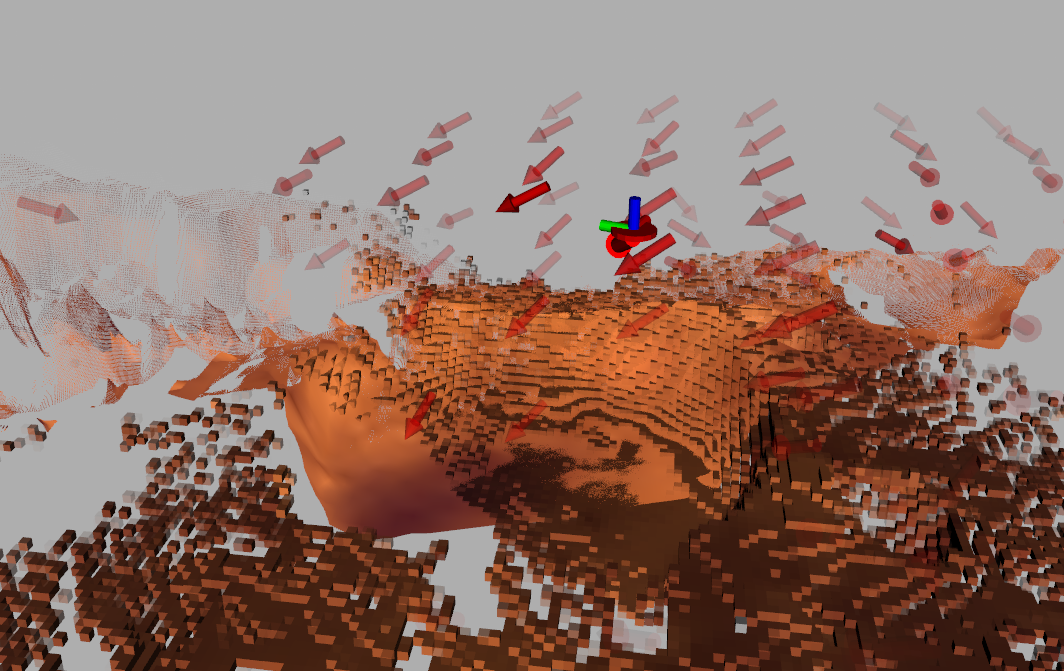
\includegraphics[width=0.9\textwidth]{mars_closeup.png}
        		\caption{Full Map Cells and Sensor Scan}
		\vspace*{0.025\textwidth}
    	\end{subfigure}
	\centering
	\begin{subfigure}[t]{0.95\columnwidth}
           	\centering
          	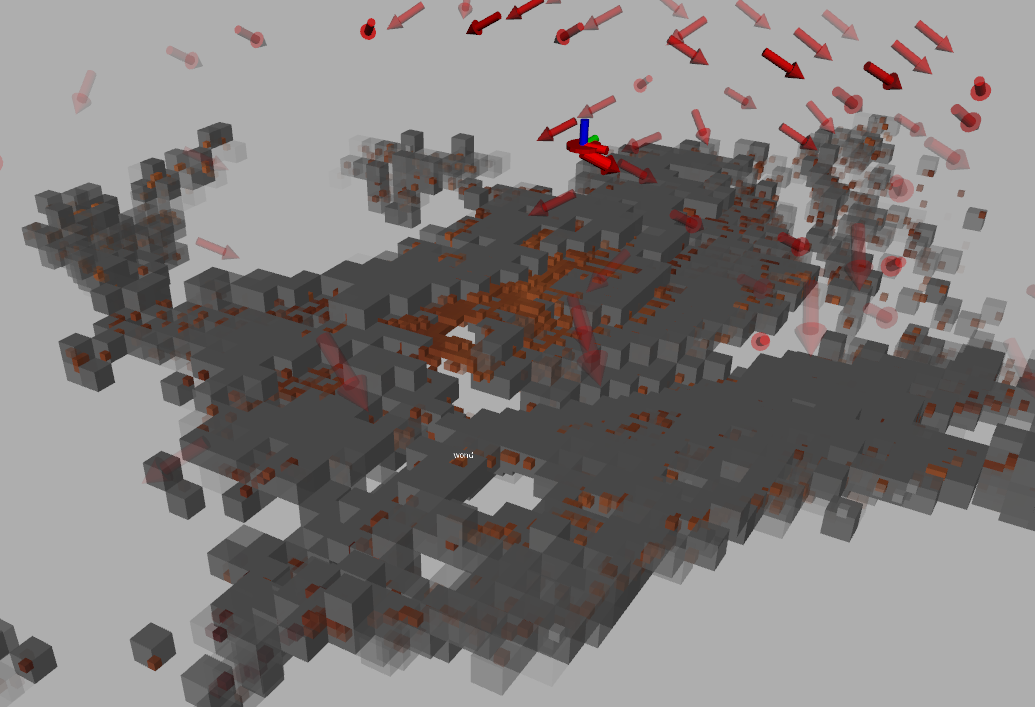
\includegraphics[width=0.9\textwidth]{scitech_reducedCells.png}
        		\caption{Full Map and Reduced Map Cells}
		\vspace*{0.025\textwidth}
    	\end{subfigure}
\caption{The close-up images from the Case 2 trial show the candidate future poses (red arrows), where greater opacity represents a larger objective function of \refeqn{CandidateLocationOptimization}. In (a), we show the 3D scan with color corresponding to the surface of Mars. In (b), we overlay the full map $m$ (colored) with the reduced map $m_\text{reduced}$ (gray) from \refeqn{Proj3DMapComb}.}
\label{fig:marsZoomedIn}
\end{figure}


	\begin{figure}
		\centerline{
			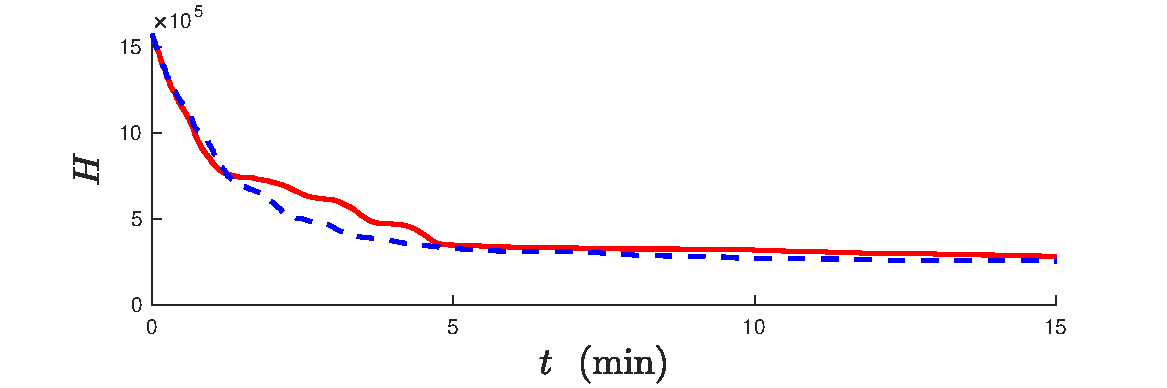
\includegraphics[width=0.6\columnwidth]{scitech_entropy_comparison_flat.pdf}
		}
		\caption{The complete map entropy for Case 1 (red solid line) decreases at roughly the same rate as the reduced map entropy for Case 2 (dashed blue line) toward the beginning. However, the expected entropy in Case 2 promotes actions toward unexplored territory, while the policy of Case 1 yields a more complete map before moving on to unexplored spaces.}
		\label{fig:mars3Dentropy}
	\end{figure}


In both cases, the robot built the 3D probabilistic map of the $2000$ cubic meter space composed of $4.74\times10^6$ grid cells. The maps were mostly complete within $10$ minutes. The $\tilde{\theta}=30^{\circ}$ downward viewing angle captured the ground nicely, as candidate attitudes tended to direct the onboard sensor toward uncertain regions on the surface of Mars. The proposed approach provided collision-free mapping and autonomous exploration in real-time.

However, the choice of occupancy grid map used for entropy predictions introduced an interesting tradeoff. In Case 1, when the full probabilistic map $m$ was used in \refeqn{Iscan}, regions where the grid cells were partially-known were frequently reconsidered until the space was well-known. Conversely in Case 2, when $m_\text{reduced}$ was used instead, the robot repeatedly left spaces that were missing a few grid cells to visit new terrain. This is because $m_\text{reduced}$ contained some cells with large occupancy probabilities based on \refeqn{Proj3DMapComb}, which allowed some grid cells of $m$ enclosed within a cell of $m_\text{reduced}$ to be uncertain. The exploration policy of Case 2 incorrectly assumed these regions were well-known. Ironically, this false assumption actually led to greater information gains when the vehicle moved on to unvisited terrain. Conversely with Case $1$, which used $m$ for computing expected entropy, the total map entropy decreased more steadily and generated a more-complete 3D occupancy grid of the surface of Mars.

In short, the proposed 3D probabilistic occupancy grid mapping and autonomous exploration were simulated successfully in real-time over the surface of Mars using ROS and Gazebo. Choosing $m$ for entropy predictions produced a more-complete map, but choosing $m_\text{reduced}$ was sometimes beneficial for exploring new terrain faster, while forgoing map completeness.



\section{Conclusions}

This chapter covers autonomous exploration through a 3D environment, such that the robot can account for complex geometries in all dimension and explore with upward and downward motions. The expected information gains are calculated with predicting the entropy changes from sample rays in 3D space, and the bump function is applied using the cost from Dijkstra's search. An example where a robot maps and explores the surface of Mars demonstrates the efficacy of the approach.



